\documentclass[aspectratio=169,10pt]{beamer}

% ============================================================
% Theme and Color Setup - Professional Research Style
% ============================================================
\usetheme{Madrid}
\usecolortheme{seahorse}

% Custom colors inspired by ICML/NeurIPS style
\definecolor{icmlblue}{RGB}{0,73,135}
\definecolor{icmlred}{RGB}{178,34,34}
\definecolor{icmlgreen}{RGB}{34,139,34}
\definecolor{icmlorange}{RGB}{255,140,0}
\definecolor{lightgray}{RGB}{245,245,245}

\setbeamercolor{structure}{fg=icmlblue}
\setbeamercolor{title}{fg=white,bg=icmlblue}
\setbeamercolor{frametitle}{fg=icmlblue,bg=lightgray}
\setbeamercolor{block title}{fg=white,bg=icmlblue}
\setbeamercolor{block body}{fg=black,bg=lightgray}
\setbeamercolor{alerted text}{fg=icmlred}
\setbeamercolor{example text}{fg=icmlgreen}

% ============================================================
% Packages
% ============================================================
\usepackage[utf8]{inputenc}
\usepackage{amsmath,amssymb,amsthm}
\usepackage{graphicx}
\graphicspath{{images/}}
\usepackage{booktabs}
\usepackage{algorithm}
\usepackage{algorithmic}
\usepackage{tikz}
\usepackage{pgfplots}
\pgfplotsset{compat=1.15}
\usetikzlibrary{shapes,arrows,positioning,calc,fit,backgrounds}

% ============================================================
% Title Information
% ============================================================
\title[HybridRoute]{HybridRoute: Cost-Optimal LLM Routing\\via Learning-Augmented Online Algorithms}
\subtitle{ICML 2026 Submission}
\author{Harvard Systems Lab}
\institute{}
\date{\today}

% ============================================================
% Document Begin
% ============================================================
\begin{document}

% ----------------------------------------------------------
% Title Slide
% ----------------------------------------------------------
\begin{frame}
\titlepage
\end{frame}

% ----------------------------------------------------------
% Outline
% ----------------------------------------------------------
\begin{frame}{Outline}
\tableofcontents
\end{frame}

% ============================================================
\section{Motivation \& Problem}
% ============================================================

% ----------------------------------------------------------
\begin{frame}{Motivation: The Rise of Hybrid Pricing Models}
    % 1. Context: Model Commoditization
    \textbf{Context:} The same model (e.g., \texttt{Llama-3-70B}, \texttt{DeepSeek-R1}) is now accessible via distinct billing paradigms:

    \vspace{0.3cm}

    \begin{columns}[T]
        \begin{column}{0.48\textwidth}
            \begin{block}{Option A: Pay-per-Token API}
                \begin{itemize}
                    \item \textbf{Example:} OpenAI, DeepSeek API
                    \item \textbf{Cost:} Linear in length ($L \times P_{\text{token}}$)
                    \item \textbf{Capacity:} Elastic / Unlimited
                    \item \textit{``High Marginal Cost''}
                \end{itemize}
            \end{block}
        \end{column}

        \begin{column}{0.48\textwidth}
            \begin{block}{Option B: Fixed-Quota Subscription}
                \begin{itemize}
                    \item \textbf{Example:} Reserved GPUs, Chutes
                    \item \textbf{Cost:} Sunk (Monthly Fee)
                    \item \textbf{Capacity:} Hard constraints (Quota/QPS)
                    \item \textit{``Zero Marginal Cost''}
                \end{itemize}
            \end{block}
        \end{column}
    \end{columns}

    \vspace{0.4cm}

    % 2. The Core Problem
    \begin{alertblock}{The Challenge: Heterogeneous Request Values}
        Not all requests maximize the value of scarce subscription slots.
        \begin{itemize}
            \item \textbf{Short Request:} Saves \$0.001 on API $\to$ \textcolor{icmlred}{Wastes Quota Opportunity}
            \item \textbf{Long Request:} Saves \$0.500 on API $\to$ \textcolor{icmlgreen}{High Value Usage}
        \end{itemize}
        \centering
        \textit{Naive routing (Greedy/FCFS) fails to capture this \textbf{Opportunity Cost}.}
    \end{alertblock}

    \vspace{0.2cm}
    \centering
    \textbf{Goal:} Route \textbf{high-value requests} to subscriptions under uncertainty.
\end{frame}

% ----------------------------------------------------------
\begin{frame}{A Unified View: Three Resource Categories}
\begin{center}
\textcolor{icmlblue}{\textbf{Why These Three Categories?}}\\[0.3cm]
\small Our abstraction captures both \textbf{API services} and \textbf{local GPU deployments}
\end{center}

\vspace{0.3cm}

\begin{columns}[T]
\begin{column}{0.32\textwidth}
\begin{block}{Concurrency-Limited ($S_C$)}
\centering
\textbf{$C$ parallel slots}
\vspace{0.2cm}

\footnotesize
\textcolor{icmlblue}{API World:}\\
Subscription with concurrency cap

\vspace{0.2cm}
\textcolor{icmlgreen}{Local Deployment:}\\
\textbf{Dedicated GPU cluster}\\
(fixed \# of serving replicas)
\end{block}
\end{column}

\begin{column}{0.32\textwidth}
\begin{block}{Daily-Quota ($S_Q$)}
\centering
\textbf{$Q$ requests/day}
\vspace{0.2cm}

\footnotesize
\textcolor{icmlblue}{API World:}\\
Free tier / subscription quota

\vspace{0.2cm}
\textcolor{icmlgreen}{Local Deployment:}\\
\textbf{Gutter Pool}\\
(spare nodes for HA)
\end{block}
\end{column}

\begin{column}{0.32\textwidth}
\begin{block}{Pay-per-Token ($S_A$)}
\centering
\textbf{Unlimited, \$/token}
\vspace{0.2cm}

\footnotesize
\textcolor{icmlblue}{API World:}\\
OpenAI, Anthropic, etc.

\vspace{0.4cm}
\textit{No capacity limit}\\
\textit{Always available}
\end{block}
\end{column}
\end{columns}

\vspace{0.4cm}
\begin{center}
\fbox{\parbox{0.85\textwidth}{
\centering
\textbf{Key Insight:} Our algorithms apply to \textit{any} system with these resource types---\\
whether routing to external APIs or scheduling across local GPU pools.
}}
\end{center}
\end{frame}

% ----------------------------------------------------------
\begin{frame}{The LLM API Pricing Landscape}
\begin{columns}[T]
\begin{column}{0.55\textwidth}
\textbf{Two Dominant Pricing Models:}
\vspace{0.3cm}

\begin{block}{Pay-per-Token API ($S_A$)}
\begin{itemize}
    \item Unlimited capacity
    \item Cost $\propto$ (input + output) tokens
    \item Example: OpenAI, Anthropic, OpenRouter
\end{itemize}
\end{block}

\begin{block}{Subscription Plans ($S_Q$, $S_C$)}
\begin{itemize}
    \item \textbf{Daily Quota} ($S_Q$): $Q$ requests/day, \$20/month
    \item \textbf{Concurrency} ($S_C$): $C$ parallel slots, \$200/month
    \item Zero marginal cost once subscribed
\end{itemize}
\end{block}
\end{column}

\begin{column}{0.4\textwidth}
\centering
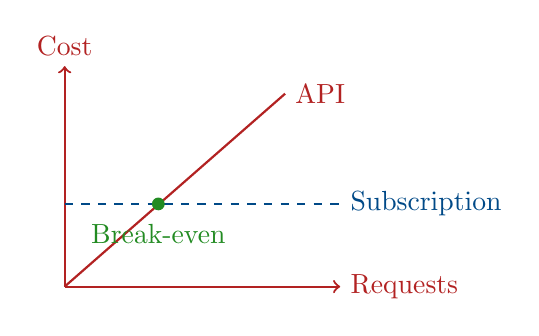
\begin{tikzpicture}[scale=0.7]
    % API cost line
    \draw[thick,icmlred,->] (0,0) -- (5,0) node[right] {Requests};
    \draw[thick,icmlred,->] (0,0) -- (0,4) node[above] {Cost};
    \draw[thick,icmlred] (0,0) -- (4,3.5) node[right] {API};

    % Subscription cost line
    \draw[thick,icmlblue,dashed] (0,1.5) -- (5,1.5) node[right] {Subscription};

    % Break-even point
    \filldraw[icmlgreen] (1.7,1.5) circle (3pt);
    \node[below,icmlgreen] at (1.7,1.3) {Break-even};
\end{tikzpicture}

\vspace{0.5cm}
\textcolor{icmlblue}{\textbf{Key Insight:}} Hybrid routing can minimize total cost!
\end{column}
\end{columns}
\end{frame}

% ----------------------------------------------------------
\begin{frame}{Research Questions}
\begin{center}
\Large
\textcolor{icmlblue}{\textbf{Core Question:}}\\[0.5cm]
\normalsize
Given a stream of LLM requests with heterogeneous costs,\\
\textbf{how should we route each request} to minimize total API spending?
\end{center}

\vspace{0.5cm}

\begin{columns}[T]
\begin{column}{0.48\textwidth}
\begin{alertblock}{Offline Setting}
\begin{itemize}
    \item Full knowledge of request trace
    \item Compute \alert{optimal lower bound}
    \item Benchmark for online algorithms
\end{itemize}
\end{alertblock}
\end{column}

\begin{column}{0.48\textwidth}
\begin{exampleblock}{Online Setting}
\begin{itemize}
    \item Requests arrive sequentially
    \item \textbf{Irrevocable} decisions
    \item Unknown future arrivals
\end{itemize}
\end{exampleblock}
\end{column}
\end{columns}
\end{frame}

% ============================================================
\section{Offline Algorithms}
% ============================================================

% ----------------------------------------------------------
\begin{frame}{Stage 1: Single Daily-Quota Subscription}
\begin{columns}[T]
\begin{column}{0.55\textwidth}
\textbf{Problem Setup:}
\begin{itemize}
    \item Providers: $S_Q$ (quota) + $S_A$ (API)
    \item $Q$ requests/day on $S_Q$ (zero cost)
    \item API cost: $c_i = \frac{n_i^{\text{in}}}{1000} p^{\text{in}} + \frac{n_i^{\text{out}}}{1000} p^{\text{out}}$
\end{itemize}

\vspace{0.3cm}
\textbf{Optimization:}
\begin{equation*}
\min \sum_{i \in \mathcal{R}} x_i^A \cdot c_i^{\text{API}}
\end{equation*}
subject to:
\begin{equation*}
\sum_{i: \text{day}(a_i)=d} x_i^Q \leq Q, \quad \forall d
\end{equation*}

\end{column}

\begin{column}{0.4\textwidth}
\begin{block}{Optimal Algorithm}
\textbf{Closed-form solution:}
\begin{enumerate}
    \item For each day $d$, collect $\mathcal{R}_d$
    \item Sort by $c_i^{\text{API}}$ descending
    \item Top-$Q$ $\rightarrow$ $S_Q$
    \item Remainder $\rightarrow$ $S_A$
\end{enumerate}
\end{block}

\vspace{0.3cm}
\textcolor{icmlgreen}{\textbf{Complexity:}} $O(n \log n)$

\vspace{0.2cm}
\textcolor{icmlblue}{\textbf{Intuition:}} Use quota on expensive requests!
\end{column}
\end{columns}
\end{frame}

% ----------------------------------------------------------
\begin{frame}{Stage 2: Dual Subscriptions (Quota + Concurrency)}
\begin{columns}[T]
\begin{column}{0.58\textwidth}
\textbf{Additional Provider:}
\begin{itemize}
    \item $S_C$: Concurrency-limited subscription
    \item At most $C$ requests executing \textbf{simultaneously}
    \item Each request $i$ occupies a slot for $p_i$ seconds
\end{itemize}

\vspace{0.3cm}
\textbf{New Constraints:}
\begin{align*}
&\text{(Concurrency)} \quad \sum_{i} \mathbf{1}[s_i \leq t < s_i + p_i] \cdot x_i^C \leq C \\
&\text{(Arrival)} \quad s_i \geq a_i \\
&\text{(Deadline)} \quad s_i + p_i \leq d_i
\end{align*}

\end{column}

\begin{column}{0.38\textwidth}
\begin{alertblock}{Complexity Result}
Stage 2 is \alert{\textbf{NP-hard}}\\[0.2cm]
\small
Couples:
\begin{itemize}
    \item Knapsack (daily quota)
    \item Parallel machine scheduling
    \item Release times + deadlines
\end{itemize}
\end{alertblock}

\vspace{0.3cm}
\begin{block}{Our Solution}
\textbf{Time-Indexed ILP}
\begin{itemize}
    \item Discretize into slots
    \item Use MIP solver (Gurobi)
    \item Exact optimal solution
\end{itemize}
\end{block}
\end{column}
\end{columns}
\end{frame}

% ----------------------------------------------------------
\begin{frame}{Stage 2: ILP Formulation}
\textbf{Time Discretization:}
\begin{itemize}
    \item Horizon: $t \in \{0, 1, \ldots, T\}$ with slot width $\Delta$
    \item Processing time: $\hat{p}_i = \lceil p_i / \Delta \rceil$ slots
    \item Valid window: $[\alpha_i, \beta_i]$ based on arrival and deadline
\end{itemize}

\vspace{0.3cm}
\begin{columns}[T]
\begin{column}{0.48\textwidth}
\textbf{Variables:}
\begin{itemize}
    \item $x_i^Q, x_i^C, x_i^A \in \{0,1\}$: routing
    \item $z_{i,t} \in \{0,1\}$: start at slot $t$
\end{itemize}

\vspace{0.2cm}
\textbf{Objective:}
\begin{equation*}
\min \sum_{i \in \mathcal{R}} x_i^A \cdot c_i^{\text{API}}
\end{equation*}
\end{column}

\begin{column}{0.48\textwidth}
\textbf{Key Constraints:}
\begin{align*}
&x_i^Q + x_i^C + x_i^A = 1 \\[0.2cm]
&\sum_{t=\alpha_i}^{\beta_i} z_{i,t} = x_i^C \\[0.2cm]
&\sum_i \sum_{\tau} z_{i,\tau} \leq C \quad \forall t
\end{align*}
\end{column}
\end{columns}
\end{frame}

% ============================================================
\section{Online Algorithms}
% ============================================================

% ----------------------------------------------------------
\begin{frame}{Online Routing: Challenges}
\begin{center}
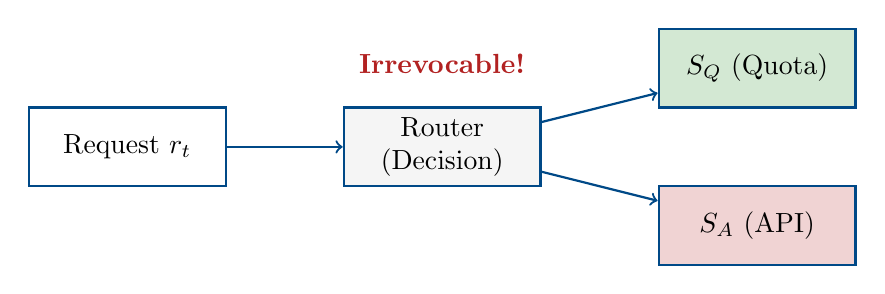
\begin{tikzpicture}[
    box/.style={rectangle, draw=icmlblue, thick, minimum width=2.5cm, minimum height=1cm, align=center},
    arrow/.style={->, thick, icmlblue}
]
    \node[box] (req) at (0,0) {Request $r_t$};
    \node[box, fill=lightgray] (router) at (4,0) {Router\\(Decision)};
    \node[box, fill=icmlgreen!20] (sq) at (8,1) {$S_Q$ (Quota)};
    \node[box, fill=icmlred!20] (sa) at (8,-1) {$S_A$ (API)};

    \draw[arrow] (req) -- (router);
    \draw[arrow] (router) -- (sq);
    \draw[arrow] (router) -- (sa);

    \node[above=0.3cm of router, text=icmlred] {\textbf{Irrevocable!}};
\end{tikzpicture}
\end{center}

\vspace{0.5cm}

\begin{columns}[T]
\begin{column}{0.48\textwidth}
\textbf{Known at Decision Time:}
\begin{itemize}
    \item Model type $m_t$
    \item Input tokens $n_t^{\text{in}}$
    \item Remaining quota $q_t$
    \item Current time $t$
\end{itemize}
\end{column}

\begin{column}{0.48\textwidth}
\textbf{Unknown:}
\begin{itemize}
    \item \alert{Output tokens} $n_t^{\text{out}}$
    \item \alert{Future requests} $r_{t+1}, r_{t+2}, \ldots$
    \item Future arrival patterns
\end{itemize}
\end{column}
\end{columns}
\end{frame}

% ----------------------------------------------------------
\begin{frame}{Online Algorithms: Greedy Baseline}
\begin{columns}[T]
\begin{column}{0.5\textwidth}
\begin{algorithm}[H]
\caption{Greedy Strategy}
\begin{algorithmic}[1]
\IF{$q_t > 0$}
    \RETURN SUBSCRIPTION
\ELSE
    \RETURN CHEAPEST\_API$(r_t)$
\ENDIF
\end{algorithmic}
\end{algorithm}

\vspace{0.3cm}
\textbf{Properties:}
\begin{itemize}
    \item Simple, no lookahead
    \item Always uses quota first
    \item \alert{May waste quota on cheap requests}
\end{itemize}
\end{column}

\begin{column}{0.45\textwidth}
\begin{exampleblock}{Cost-Aware Variant}
\begin{algorithmic}[1]
\STATE $\hat{c}_t \gets$ EstimateCost$(r_t)$
\STATE $\theta \gets \frac{\text{Monthly Fee}}{30 \times Q}$
\IF{$\hat{c}_t > \theta$ \AND $q_t > 0$}
    \RETURN SUBSCRIPTION
\ELSE
    \RETURN API
\ENDIF
\end{algorithmic}
\end{exampleblock}

\vspace{0.2cm}
\textcolor{icmlblue}{\textbf{Threshold:}} Route to subscription only if estimated API cost exceeds threshold
\end{column}
\end{columns}
\end{frame}

% ----------------------------------------------------------
\begin{frame}{Primal-Dual Threshold Strategy}
\begin{columns}[T]
\begin{column}{0.52\textwidth}
\textbf{Core Insight:} Quota is a \alert{scarce resource}---assign it an \textbf{Opportunity Cost}!

\vspace{0.3cm}
\begin{block}{Shadow Price = Opportunity Cost}
The threshold $\psi(z)$ represents the \textbf{marginal value} of the next quota slot:
\begin{equation*}
\psi(z) = L \cdot \left(\frac{U}{L}\right)^z
\end{equation*}
\begin{itemize}
    \item $z = k/Q$: fraction of quota consumed
    \item $L, U$: min/max request value bounds
    \item $\psi(z) \uparrow$ as quota becomes scarcer
\end{itemize}
\end{block}

\vspace{0.2cm}
\textbf{Decision Rule:}
\begin{equation*}
\text{Route to } S_Q \iff \underbrace{\hat{v}_t}_{\text{value}} \geq \underbrace{\psi(z)}_{\text{opp. cost}} \text{ and } k < Q
\end{equation*}
\end{column}

\begin{column}{0.44\textwidth}
\begin{exampleblock}{Economic Intuition}
\begin{itemize}
    \item \textbf{Abundant quota} ($z \to 0$):\\
    Low opportunity cost $\to$ accept freely
    \item \textbf{Scarce quota} ($z \to 1$):\\
    High opportunity cost $\to$ be selective
    \item Smooth transition via exponential
\end{itemize}
\end{exampleblock}

\vspace{0.3cm}
\begin{alertblock}{Theoretical Guarantee}
Competitive ratio: $O(\ln(U/L) + 1)$\\
\small (Optimal for online knapsack with prices)
\end{alertblock}
\end{column}
\end{columns}
\end{frame}

% ----------------------------------------------------------
\begin{frame}{Threshold Visualization: Adaptive Resource Pricing}
\begin{columns}[T]
\begin{column}{0.48\textwidth}
\centering
\textbf{Threshold vs Quota Usage}
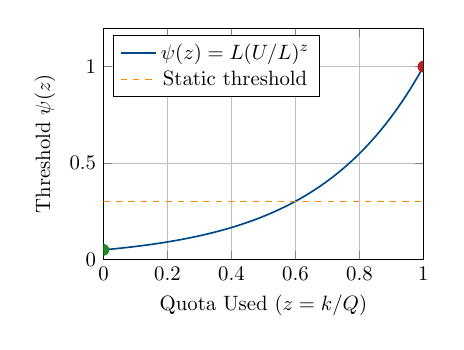
\begin{tikzpicture}[scale=0.75]
\begin{axis}[
    xlabel={Quota Used ($z = k/Q$)},
    ylabel={Threshold $\psi(z)$},
    xmin=0, xmax=1,
    ymin=0, ymax=1.2,
    grid=major,
    legend pos=north west,
    width=7cm,
    height=5.5cm,
]
% Exponential threshold: psi(z) = L * (U/L)^z
% With L=0.05, U=1.0: psi(z) = 0.05 * 20^z
\addplot[domain=0:1, samples=50, thick, icmlblue] {0.05 * (20^x)};
\addlegendentry{$\psi(z) = L(U/L)^z$}

% Constant threshold for comparison
\addplot[domain=0:1, dashed, thick, icmlorange] {0.3};
\addlegendentry{Static threshold}

% Mark L and U
\node[circle, fill=icmlgreen, inner sep=2pt] at (axis cs:0,0.05) {};
\node[left, font=\small] at (axis cs:0,0.05) {$L$};
\node[circle, fill=icmlred, inner sep=2pt] at (axis cs:1,1.0) {};
\node[right, font=\small] at (axis cs:1,1.0) {$U$};
\end{axis}
\end{tikzpicture}
\end{column}

\begin{column}{0.48\textwidth}
\textbf{Intuition:}
\begin{enumerate}
    \item \textcolor{icmlgreen}{\textbf{Abundant quota}} ($z \to 0$):\\
    Accept cheap requests (threshold $\approx L$)

    \vspace{0.2cm}
    \item \textcolor{icmlorange}{\textbf{Moderate usage}} ($z \approx 0.5$):\\
    Be selective (threshold grows)

    \vspace{0.2cm}
    \item \textcolor{icmlred}{\textbf{Scarce quota}} ($z \to 1$):\\
    Only expensive requests (threshold $\approx U$)
\end{enumerate}

\vspace{0.3cm}
\fbox{\parbox{0.9\textwidth}{
\centering
\small
\textbf{Key:} Threshold adapts to\\resource scarcity in real-time
}}
\end{column}
\end{columns}
\end{frame}

% ----------------------------------------------------------
\begin{frame}{Learning-Augmented Primal-Dual (LA-PD)}
\begin{columns}[T]
    \begin{column}{0.5\textwidth}
        \textbf{The Idea:} Route based on \textbf{Conservative Value Estimates}.

        \vspace{0.4cm}

        % Visualization of Quantile Prediction
        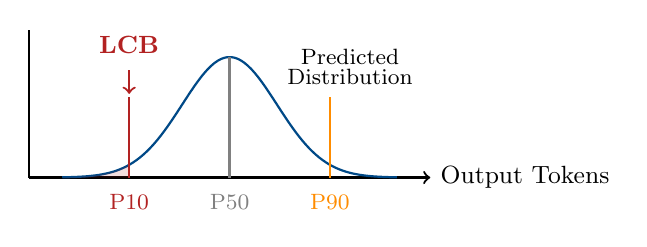
\begin{tikzpicture}[scale=0.85]
            % Axis
            \draw[->, thick] (0,0) -- (6,0) node[right] {\small Output Tokens};
            \draw[-, thick] (0,0) -- (0,2.2);

            % Distribution Curve (Bell shape)
            \draw[thick, icmlblue, domain=0.5:5.5, samples=100] plot (\x, {1.8*exp(-(\x-3)^2)});

            % Quantiles
            \draw[thick, icmlred] (1.5, 0) -- (1.5, 1.2);
            \node[below, icmlred, font=\footnotesize] at (1.5, -0.1) {P10};

            \draw[thick, gray] (3.0, 0) -- (3.0, 1.8);
            \node[below, gray, font=\footnotesize] at (3.0, -0.1) {P50};

            \draw[thick, icmlorange] (4.5, 0) -- (4.5, 1.2);
            \node[below, icmlorange, font=\footnotesize] at (4.5, -0.1) {P90};

            % Conservative Region
            \fill[icmlred, opacity=0.15] (0.5,0) -- plot[domain=0.5:1.5] (\x, {1.8*exp(-(\x-3)^2)}) -- (1.5,0) -- cycle;

            % Arrow pointing to LCB
            \draw[->, thick, icmlred] (1.5, 1.6) -- (1.5, 1.25);
            \node[above, font=\small, align=center, icmlred] at (1.5, 1.7) {\textbf{LCB}};

            % Label
            \node[font=\footnotesize, align=left] at (4.8, 1.8) {Predicted};
            \node[font=\footnotesize, align=left] at (4.8, 1.5) {Distribution};
        \end{tikzpicture}

        \vspace{0.3cm}
        \small
        \textbf{LCB (Lower Confidence Bound):} Use P10 to avoid\\
        over-estimating value $\to$ prevents quota waste.
    \end{column}

    \begin{column}{0.48\textwidth}
        \begin{exampleblock}{Risk-Aware Decision Rule}
        \begin{algorithmic}[1]
        \STATE $\hat{v}_{\text{LCB}} \gets$ Predictor.P10$(r_t)$
        \STATE $\theta \gets \psi(k/Q)$ \COMMENT{Shadow Price}

        \IF{$\hat{v}_{\text{LCB}} \geq \theta$ \AND $k < Q$}
            \RETURN SUBSCRIPTION
        \ELSE
            \RETURN API
        \ENDIF
        \end{algorithmic}
        \end{exampleblock}

        \vspace{0.2cm}
        \begin{alertblock}{Why It Works}
        \begin{itemize}
            \item \textbf{High Variance?} LCB $\ll$ Median\\
            $\to$ Uncertain value $\to$ Use API (safe)
            \item \textbf{Low Variance?} LCB $\approx$ Median\\
            $\to$ Confident value $\to$ Use $S_Q$
        \end{itemize}
        \end{alertblock}
    \end{column}
\end{columns}
\end{frame}

% ============================================================
\section{Experiments}
% ============================================================

% ----------------------------------------------------------
\begin{frame}{Experimental Setup}
\begin{columns}[T]
\begin{column}{0.5\textwidth}
\textbf{Datasets:}
\begin{table}[h]
\footnotesize
\begin{tabular}{lcc}
\toprule
Dataset & Requests & Days \\
\midrule
ShareGPT & 201K & 7 \\
FreeInference & 371K & 90 \\
RedNote & 55K & 84 \\
\bottomrule
\end{tabular}
\end{table}

\vspace{0.2cm}
\textbf{Provider Configuration:}
\begin{itemize}
    \item $S_Q$: Daily quota, \$20/month
    \item $S_A$: Pay-per-token (multi-model pricing)
\end{itemize}
\end{column}

\begin{column}{0.45\textwidth}
\textbf{Strategies Compared:}
\begin{enumerate}
    \item \textbf{All-API}: Upper bound (no subscription)
    \item \textbf{Greedy}: Use quota first-come-first-served
    \item \textbf{Optimal}: Offline oracle (sort by cost)
    \item \textbf{Primal-Dual}: Online threshold-based
\end{enumerate}

\vspace{0.3cm}
\textbf{Metrics:}
\begin{itemize}
    \item API cost savings (\%)
    \item Competitive ratio: $\frac{\text{Greedy Cost}}{\text{Optimal Cost}}$
\end{itemize}
\end{column}
\end{columns}
\end{frame}

% ----------------------------------------------------------
\begin{frame}{Offline Results: Stage 1 (Quota-Only)}
\begin{columns}[T]
\begin{column}{0.5\textwidth}
\begin{table}[h]
\footnotesize
\centering
\begin{tabular}{lcccc}
\toprule
Dataset & Type & Greedy & Optimal & CR \\
\midrule
ShareGPT & single & 17\% & \textbf{35\%} & 1.43x \\
FreeInference & multi & 63\% & \textbf{82\%} & 1.36x \\
RedNote & multi & 81\% & \textbf{98\%} & 4.36x \\
\bottomrule
\end{tabular}
\caption{API cost savings vs All-API (DeepSeek-R1 pricing)}
\end{table}

\vspace{0.3cm}
\textbf{Key Observations:}
\begin{itemize}
    \item Optimal saves \textbf{35--98\%} API costs
    \item Greedy leaves \textbf{18--20\%} on the table
    \item RedNote: High variance $\Rightarrow$ large gap
\end{itemize}
\end{column}

\begin{column}{0.45\textwidth}
\centering
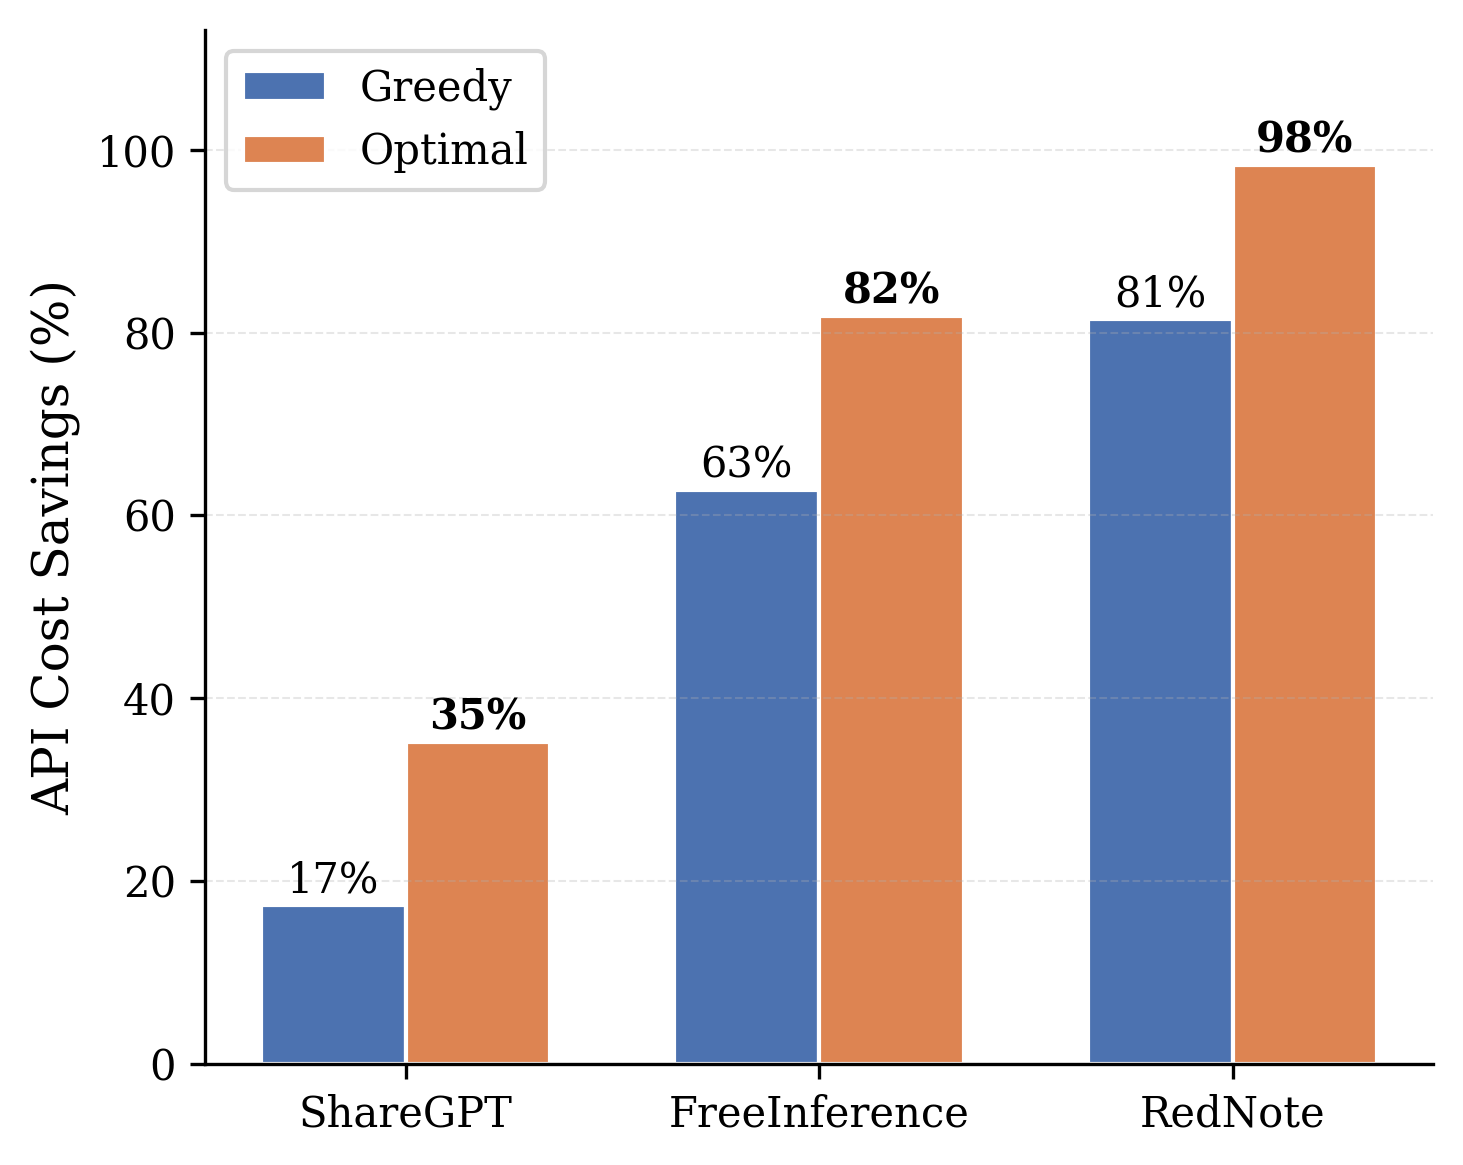
\includegraphics[width=\textwidth]{cost_savings.png}

\vspace{0.2cm}
\small
\textcolor{icmlblue}{\textbf{Takeaway:}} Optimal routing doubles the savings on some workloads!
\end{column}
\end{columns}
\end{frame}

% ----------------------------------------------------------
\begin{frame}{Stage 1: Competitive Ratio (Greedy vs Optimal)}
\begin{columns}[T]
\begin{column}{0.55\textwidth}
\centering
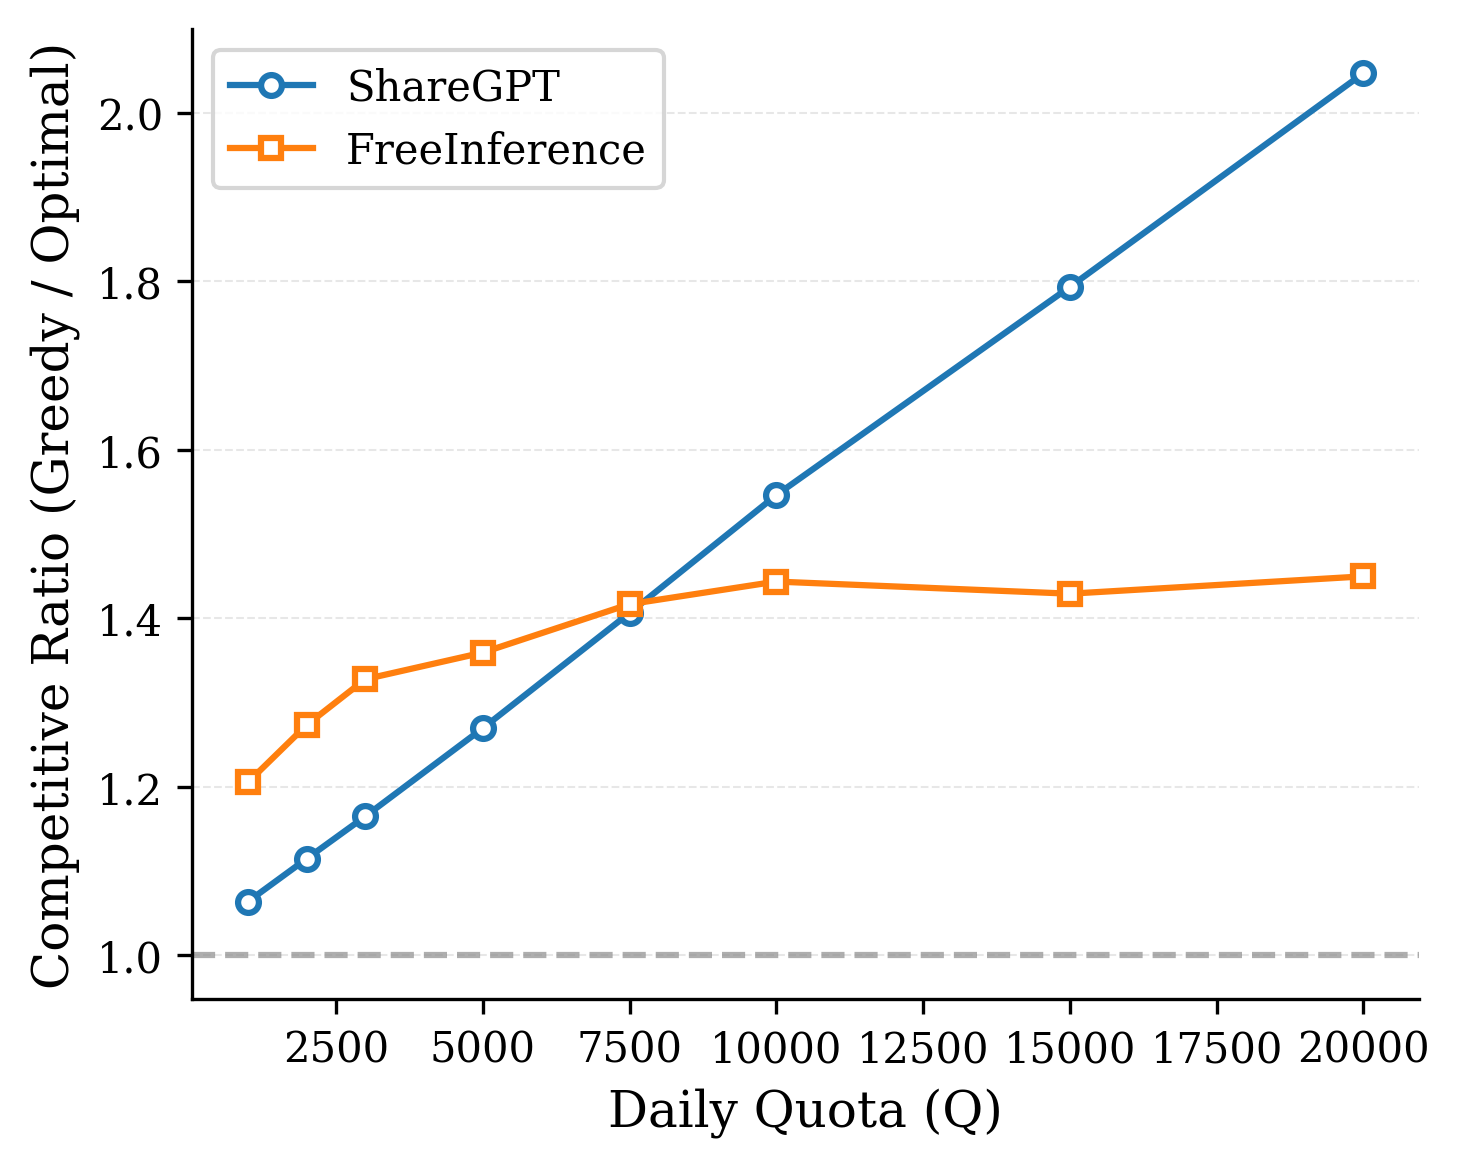
\includegraphics[width=\textwidth]{competitive_ratio.png}
\end{column}

\begin{column}{0.4\textwidth}
\textbf{Key Findings:}
\begin{itemize}
    \item Greedy is \textbf{1.2--2.0x} worse than Optimal
    \item Gap varies by workload characteristics
    \item \alert{Opportunity for online algorithms!}
\end{itemize}

\vspace{0.3cm}
\textbf{Why the Gap?}
\begin{itemize}
    \item Greedy wastes quota on cheap requests
    \item Optimal selects highest-value requests
    \item Cost distribution matters
\end{itemize}
\end{column}
\end{columns}
\end{frame}

% ----------------------------------------------------------
\begin{frame}{Stage 1: Sensitivity Analysis (Cost vs Quota)}
\begin{columns}[T]
\begin{column}{0.48\textwidth}
\centering

\includegraphics[width=\textwidth]{fig2_sensitivity_sharegpt.png}
\vspace{0.1cm}
\small ShareGPT (single-model)
\end{column}

\begin{column}{0.48\textwidth}
\centering

\includegraphics[width=\textwidth]{fig2_sensitivity_freeinference.png}
\vspace{0.1cm}
\small FreeInference (multi-model)
\end{column}
\end{columns}

\vspace{0.3cm}
\begin{center}
\textbf{Key Insight:} The gap between Greedy and Optimal \textbf{widens} as quota increases.\\
\small Shaded area = potential savings from optimal routing
\end{center}
\end{frame}

% ----------------------------------------------------------
\begin{frame}{Online Results: Cost Comparison}
\begin{columns}[T]
\begin{column}{0.55\textwidth}
\centering
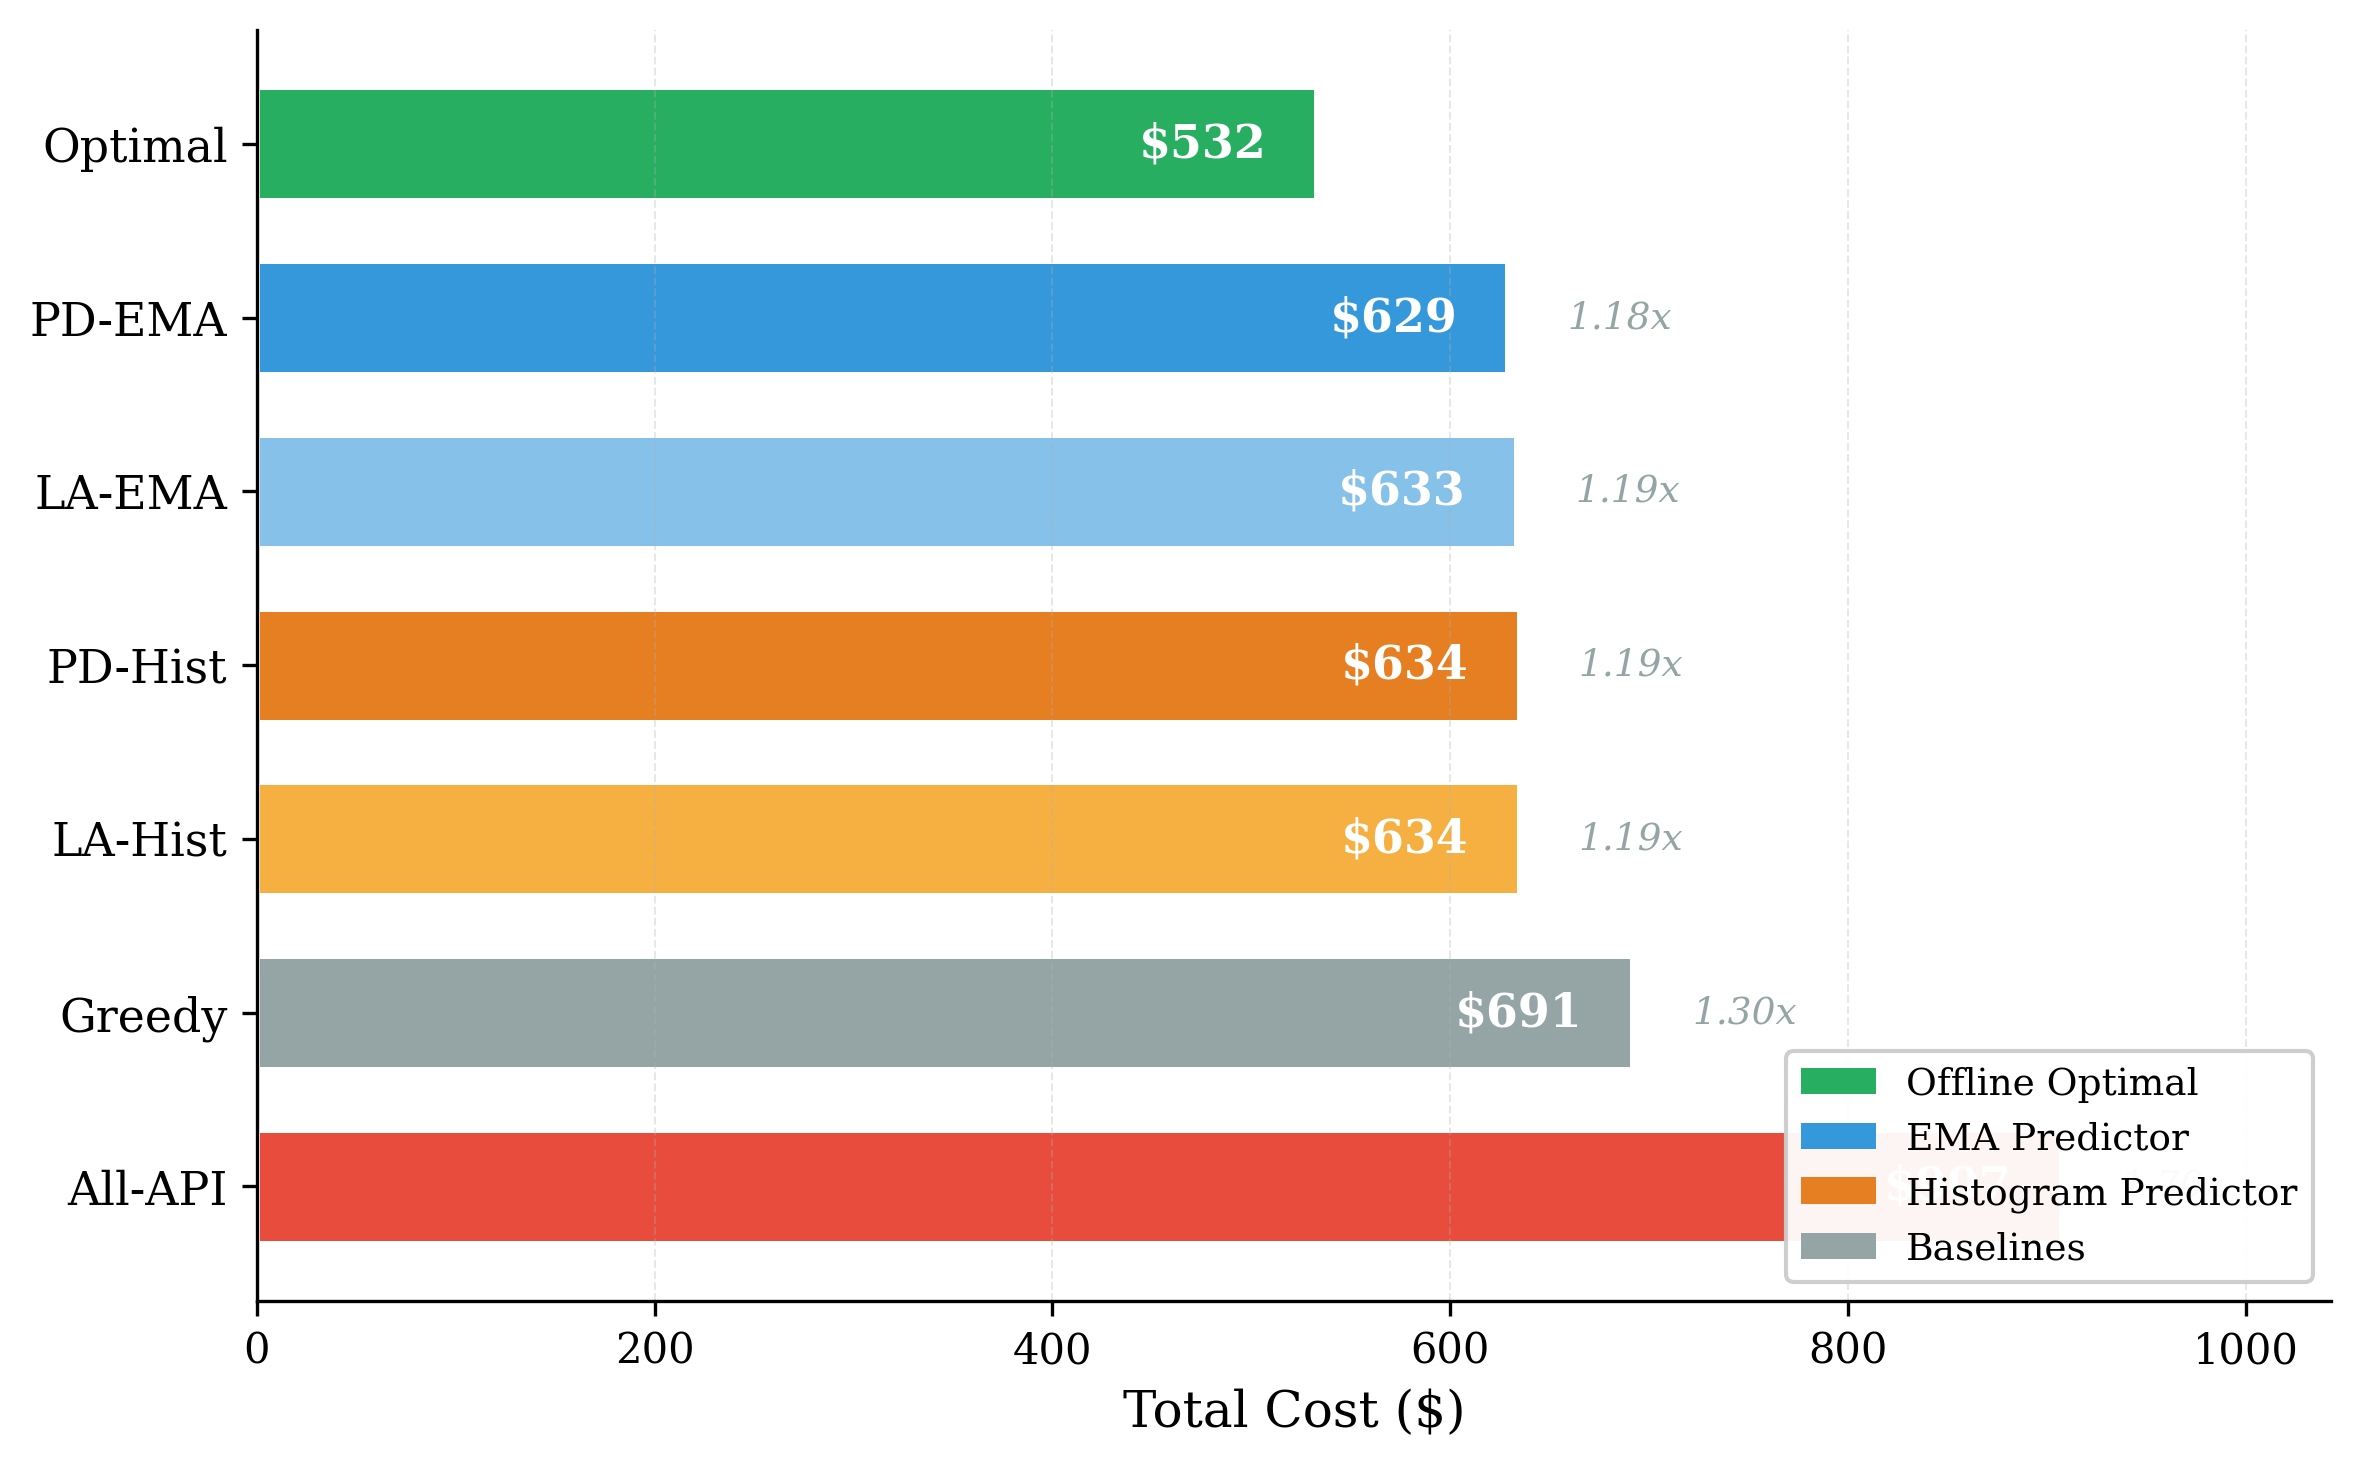
\includegraphics[width=\textwidth]{online_cost_comparison.png}
\end{column}

\begin{column}{0.42\textwidth}
\textbf{BurstGPT Dataset:}
\begin{itemize}
    \item 1.4M requests, 61 days
    \item DeepSeek-R1 pricing
    \item Daily quota $Q = 5000$
\end{itemize}

\vspace{0.3cm}
\begin{table}[h]
\footnotesize
\centering
\begin{tabular}{lcc}
\toprule
Strategy & Cost & CR \\
\midrule
All-API & \$907 & 1.70x \\
Greedy & \$691 & 1.30x \\
\textbf{PD-EMA} & \textcolor{icmlgreen}{\textbf{\$629}} & \textbf{1.18x} \\
LA-EMA & \$633 & 1.19x \\
Optimal & \$532 & 1.00x \\
\bottomrule
\end{tabular}
\end{table}

\vspace{0.2cm}
\fbox{\parbox{0.95\textwidth}{
\centering
\small
\textbf{30\% savings} vs All-API\\
\textbf{9\% better} than Greedy
}}
\end{column}
\end{columns}
\end{frame}

% ----------------------------------------------------------
\begin{frame}{Ablation Study: Predictor vs Decision Rule}
\begin{columns}[T]
    \begin{column}{0.48\textwidth}
        \centering
        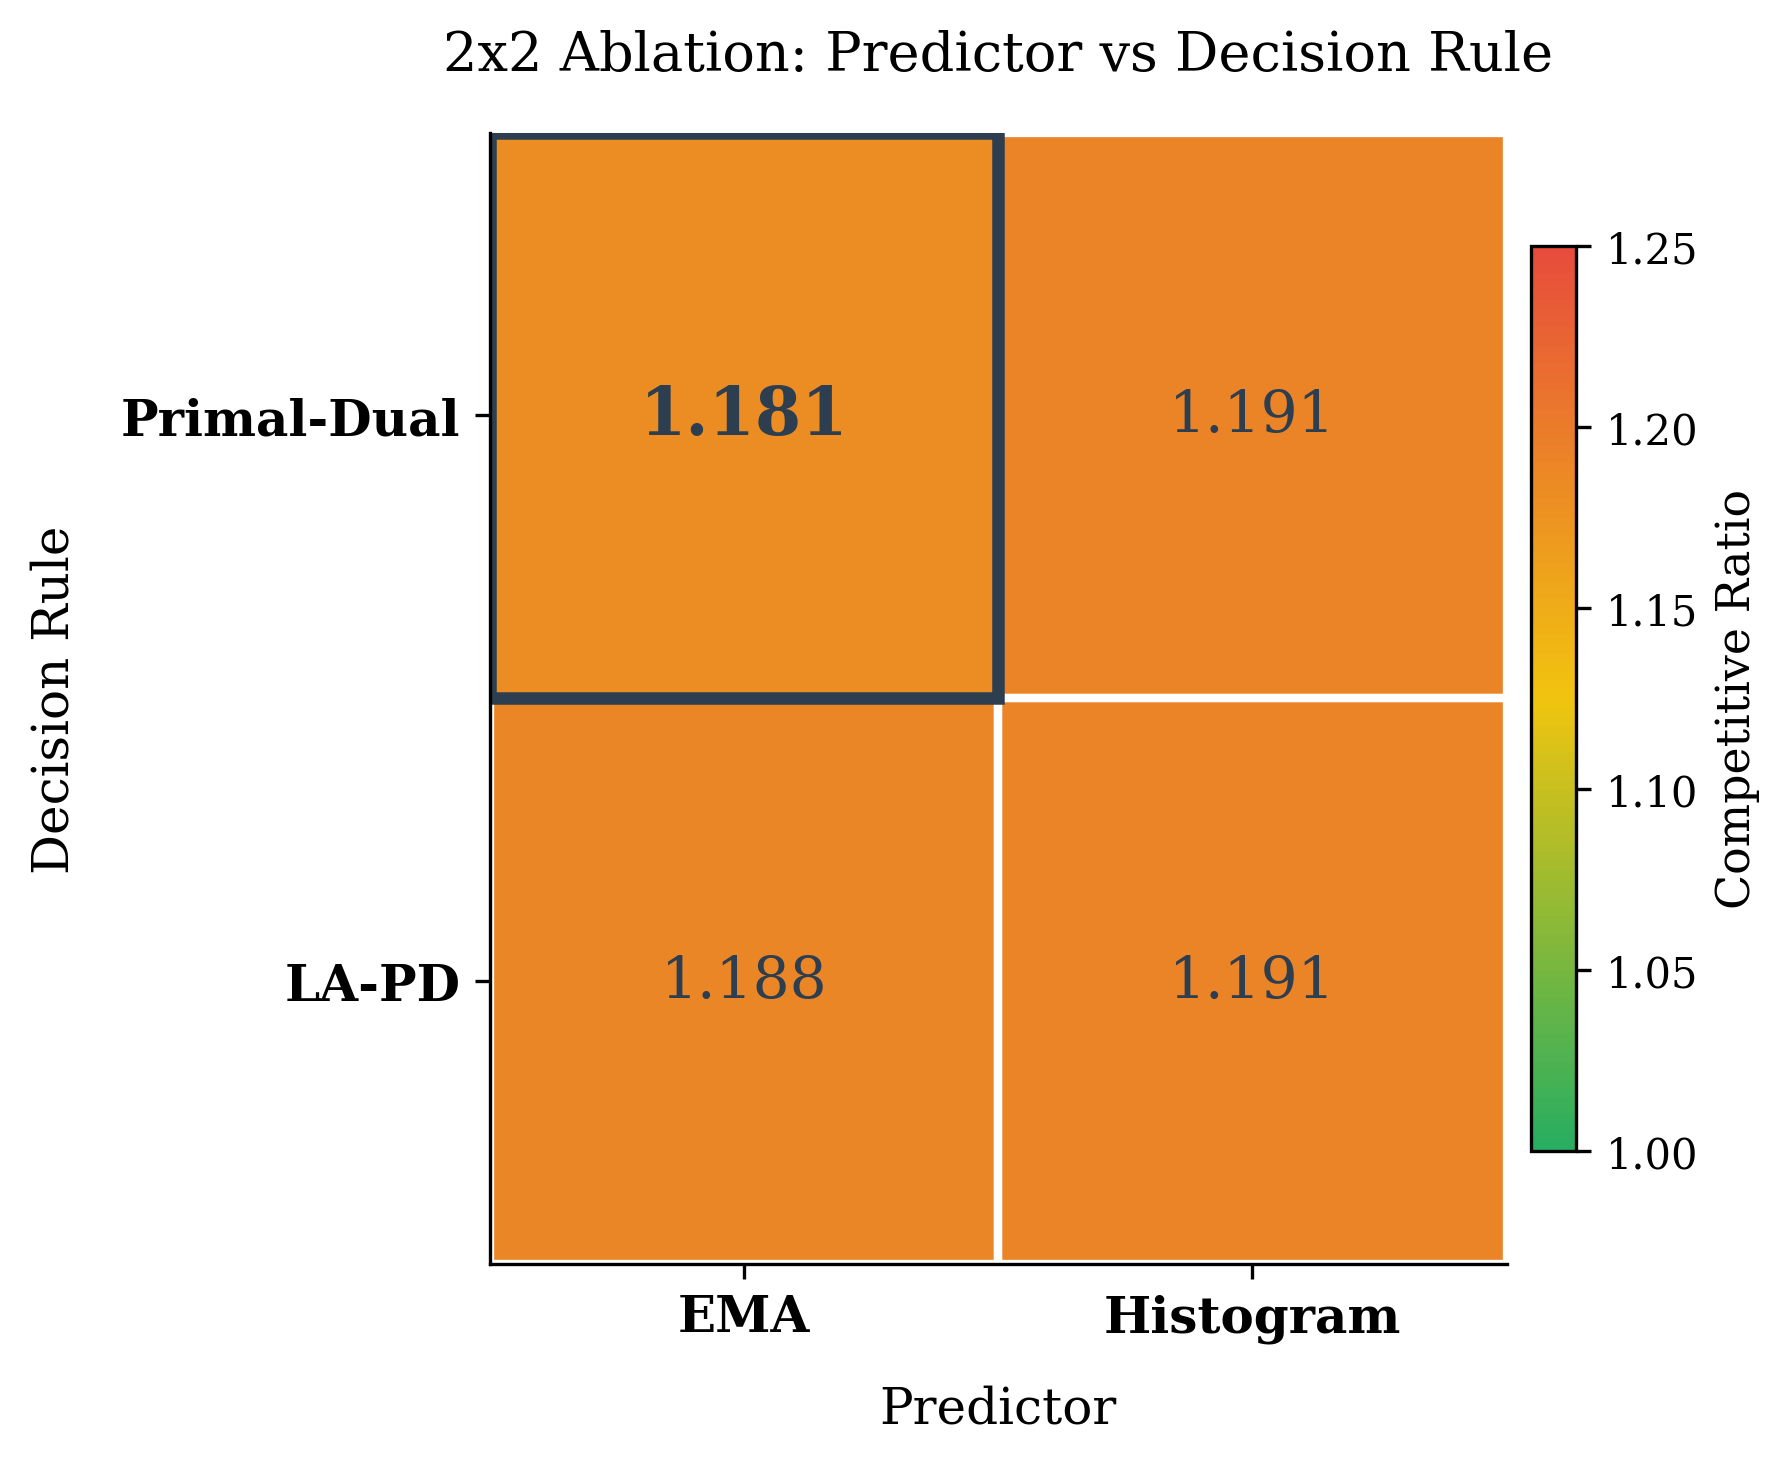
\includegraphics[width=0.95\textwidth]{online_ablation_heatmap.png}

        \vspace{0.2cm}
        \small
        \textbf{2$\times$2 Factorial Design:}\\
        Predictor $\times$ Decision Rule
    \end{column}

    \begin{column}{0.48\textwidth}
        \textbf{Key System Insights:}

        \vspace{0.2cm}

        \begin{block}{1. Predictor Dominance}
        \alert{Predictor quality $>$ rule complexity.}
        \begin{itemize}
            \item Switching Hist $\to$ EMA improves CR more than switching PD $\to$ LA.
        \end{itemize}
        \end{block}

        \vspace{0.15cm}

        \begin{block}{2. The Power of Simplicity}
        \textbf{EMA outperforms Histogram.} Why?
        \begin{itemize}
            \item Faster adaptation to non-stationary arrivals
            \item Better data efficiency (fewer samples to warm up)
        \end{itemize}
        \end{block}

        \vspace{0.15cm}

        \fbox{\parbox{0.95\textwidth}{
        \centering
        \small
        \textbf{Lesson:} In online systems,\\
        \textit{lightweight adaptivity $>$ complex modeling}
        }}
    \end{column}
\end{columns}
\end{frame}

% ----------------------------------------------------------
\begin{frame}{Predictor Calibration Analysis}
\begin{columns}[T]
\begin{column}{0.52\textwidth}
\centering

\includegraphics[width=\textwidth]{online_calibration.png}
\end{column}

\begin{column}{0.45\textwidth}
\textbf{Calibration Metric:}
\[
\text{Coverage}_\tau = P(\text{actual} \leq \hat{q}_\tau)
\]
Ideal: Coverage$_\tau = \tau$

\vspace{0.3cm}
\textbf{Results:}
\begin{itemize}
    \item \textbf{Histogram}: Better calibrated
    \begin{itemize}
        \item q50: 56\% (ideal: 50\%)
    \end{itemize}
    \item \textbf{EMA}: Over-estimates
    \begin{itemize}
        \item q50: 72\% (ideal: 50\%)
    \end{itemize}
\end{itemize}

\vspace{0.2cm}
\begin{alertblock}{Paradox Explained}
\small
Better calibration $\neq$ better cost!\\
EMA's point estimate is more accurate for \textit{routing decisions}.
\end{alertblock}
\end{column}
\end{columns}
\end{frame}

% ----------------------------------------------------------
\begin{frame}{Stage 2 Results: Quota + Concurrency (Zero-Wait)}
\begin{columns}[T]
\begin{column}{0.52\textwidth}
\centering
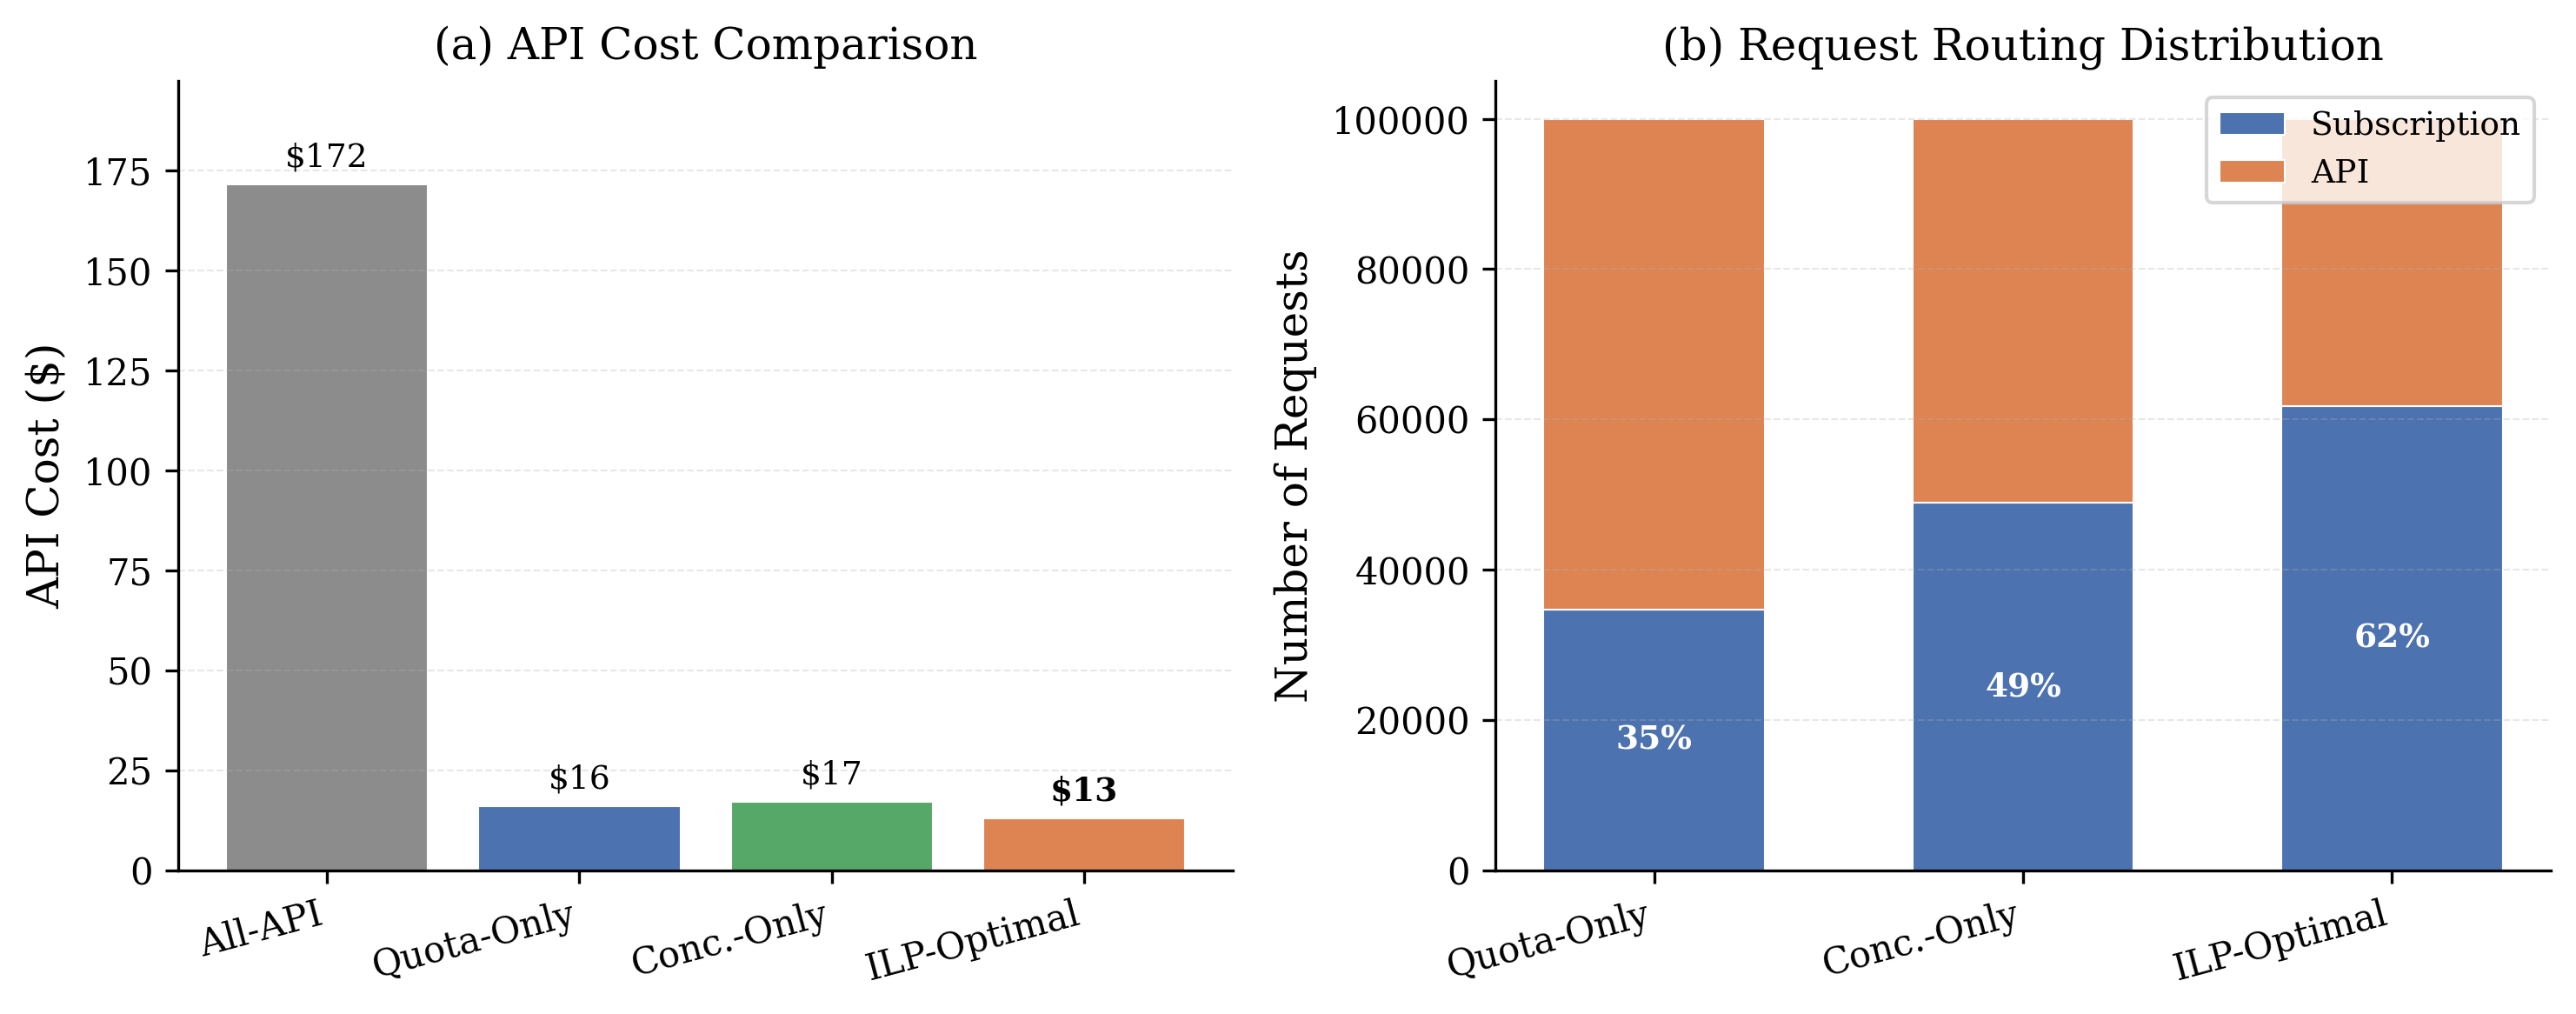
\includegraphics[width=\textwidth]{stage2_combined.png}

\vspace{0.2cm}
\small
RedNote Dataset: 55K requests, 84 days\\
Zero-wait semantics (no queueing)
\end{column}

\begin{column}{0.45\textwidth}
\textbf{System Semantics:}
\begin{itemize}
    \item \textbf{Zero-wait / Loss system}: requests cannot queue
    \item If $S_C$ is full at arrival $\to$ route to API immediately
\end{itemize}

\vspace{0.3cm}
\begin{table}[h]
\footnotesize
\centering
\begin{tabular}{lcc}
\toprule
Strategy & API Cost & Sub Reqs \\
\midrule
Quota-Only & \$8,338 & 6,731 \\
Conc.-Only & \$8,496 & 639 \\
Greedy & \$8,361 & 7,616 \\
\textbf{ILP-Opt} & \textcolor{icmlgreen}{\textbf{\$8,333}} & 6,988 \\
\bottomrule
\end{tabular}
\end{table}

\vspace{0.2cm}
\begin{alertblock}{Key Insight}
\small
Under zero-wait, \textbf{quota dominates concurrency}.\\
Joint optimization yields marginal gain (+0.05\%).
\end{alertblock}
\end{column}
\end{columns}
\end{frame}

% ----------------------------------------------------------
\begin{frame}{Stage 2: Single-Model Comparison}
\begin{columns}[T]
\begin{column}{0.55\textwidth}
\centering

\includegraphics[width=\textwidth]{single_model_comparison_rednote.png}

\vspace{0.2cm}
\small
Model size affects effective concurrency:\\
Large models ($4\times$ weight) $\to$ fewer concurrent slots
\end{column}

\begin{column}{0.42\textwidth}
\textbf{Model Size Impact:}
\begin{itemize}
    \item \textbf{Small} (mult=1): $C_{\text{eff}}=8$
    \item \textbf{Medium} (mult=2): $C_{\text{eff}}=4$
    \item \textbf{Large} (mult=4): $C_{\text{eff}}=2$
\end{itemize}

\vspace{0.3cm}
\begin{exampleblock}{Observations}
\begin{itemize}
    \item Larger models $\to$ concurrency less effective
    \item Quota-Only remains competitive across sizes
    \item ILP finds best allocation per model
\end{itemize}
\end{exampleblock}

\vspace{0.2cm}
\fbox{\parbox{0.95\textwidth}{
\centering
\small
\textbf{Takeaway:} Model size determines\\
optimal quota vs concurrency balance
}}
\end{column}
\end{columns}
\end{frame}

% ============================================================
\section{Latency-Aware Routing}
% ============================================================

% ----------------------------------------------------------
\begin{frame}{Motivation: Beyond Cost---Latency SLO Matters}
\begin{columns}[T]
\begin{column}{0.52\textwidth}
\textbf{The Problem:}
\begin{itemize}
    \item OpenRouter aggregates \textbf{12+ providers} for the same model
    \item Each provider has \alert{different latency distributions}
    \item Users have \textbf{Service Level Objectives} (SLO)
    \item \textit{e.g., ``99\% of requests complete in $<$2 seconds''}
\end{itemize}

\vspace{0.3cm}
\begin{alertblock}{Challenge}
How to route requests to \textbf{minimize cost} while \textbf{guaranteeing latency SLO}?
\end{alertblock}
\end{column}

\begin{column}{0.45\textwidth}
\centering
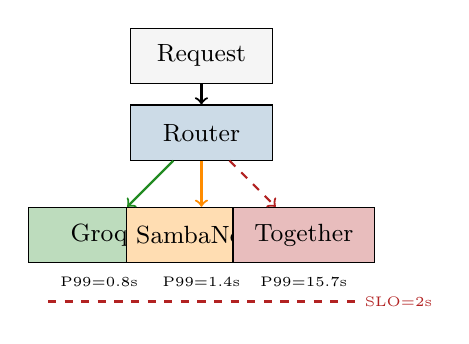
\begin{tikzpicture}[scale=0.65,
    provider/.style={rectangle, draw, minimum width=1.8cm, minimum height=0.7cm, font=\small}
]
    % Request
    \node[provider, fill=lightgray] (req) at (0,0) {Request};

    % Router
    \node[provider, fill=icmlblue!20] (router) at (0,-1.5) {Router};

    % Providers
    \node[provider, fill=icmlgreen!30] (p1) at (-2,-3.5) {Groq};
    \node[provider, fill=icmlorange!30] (p2) at (0,-3.5) {SambaNova};
    \node[provider, fill=icmlred!30] (p3) at (2,-3.5) {Together};

    % Labels
    \node[below=0.05cm of p1, font=\tiny] {P99=0.8s};
    \node[below=0.05cm of p2, font=\tiny] {P99=1.4s};
    \node[below=0.05cm of p3, font=\tiny] {P99=15.7s};

    % Arrows
    \draw[->, thick] (req) -- (router);
    \draw[->, thick, icmlgreen] (router) -- (p1);
    \draw[->, thick, icmlorange] (router) -- (p2);
    \draw[->, thick, icmlred, dashed] (router) -- (p3);

    % SLO line
    \draw[thick, icmlred, dashed] (-3,-4.8) -- (3,-4.8);
    \node[right, font=\tiny, text=icmlred] at (3,-4.8) {SLO=2s};
\end{tikzpicture}

\vspace{0.2cm}
\small
\textcolor{icmlblue}{\textbf{Key Insight:}} Provider latency varies by \textbf{20x}!
\end{column}
\end{columns}
\end{frame}

% ----------------------------------------------------------
\begin{frame}{Phase 1: Latency Profiling (12 Providers, 24h)}
\vspace{-0.3cm}
\begin{columns}[T]
\begin{column}{0.48\textwidth}
\centering

\includegraphics[width=0.95\textwidth,height=0.5\textheight,keepaspectratio]{provider_latency_cdf.png}

\scriptsize
ECDF of TTFT across 12 providers
\end{column}

\begin{column}{0.5\textwidth}
\scriptsize
\textbf{Data:} \texttt{llama-3.3-70b}, 24h, \textbf{132,900} requests, 12 providers

\vspace{0.15cm}
\begin{tabular}{lcc}
\toprule
Provider & P99 & Cost/1K \\
\midrule
\textcolor{icmlgreen}{Groq} & \textbf{796ms} & \$0.69 \\
\textcolor{icmlgreen}{SambaNova} & 1.4s & \$0.68 \\
Parasail & 4.2s & \$0.21 \\
\textcolor{icmlred}{Together} & 15.7s & \$0.88 \\
\bottomrule
\end{tabular}

\vspace{0.2cm}
\textbf{Key Insight:} P99 latency varies \textbf{20x} across providers!

\vspace{0.15cm}
\textbf{Implication:}
\begin{itemize}\setlength{\itemsep}{0pt}
    \item Fast providers (Groq) cost more
    \item Cheap providers (Parasail) have high tail latency
    \item \alert{Opportunity for cost-latency tradeoff}
\end{itemize}
\end{column}
\end{columns}
\end{frame}

% ----------------------------------------------------------
\begin{frame}{Phase 2: LP-Based Optimal Provider Mixing}
\begin{columns}[T]
\begin{column}{0.5\textwidth}
\textbf{Formulation:}
\begin{equation*}
\min_{\pi} \sum_{j} \pi_j \cdot c_j \quad \text{(Expected Cost)}
\end{equation*}
subject to:
\begin{equation*}
\sum_{j} \pi_j \cdot F_j(L) \geq 0.99 \quad \text{(P99 SLO)}
\end{equation*}
\begin{equation*}
\sum_{j} \pi_j = 1, \quad \pi_j \geq 0
\end{equation*}

\vspace{0.2cm}
\textbf{Key Insight:}
\begin{itemize}
    \item LP relaxation of provider selection
    \item $F_j(L)$ = empirical CDF at SLO $L$
    \item \alert{At most 2 providers} at optimal (LP vertex)
\end{itemize}
\end{column}

\begin{column}{0.48\textwidth}
\centering
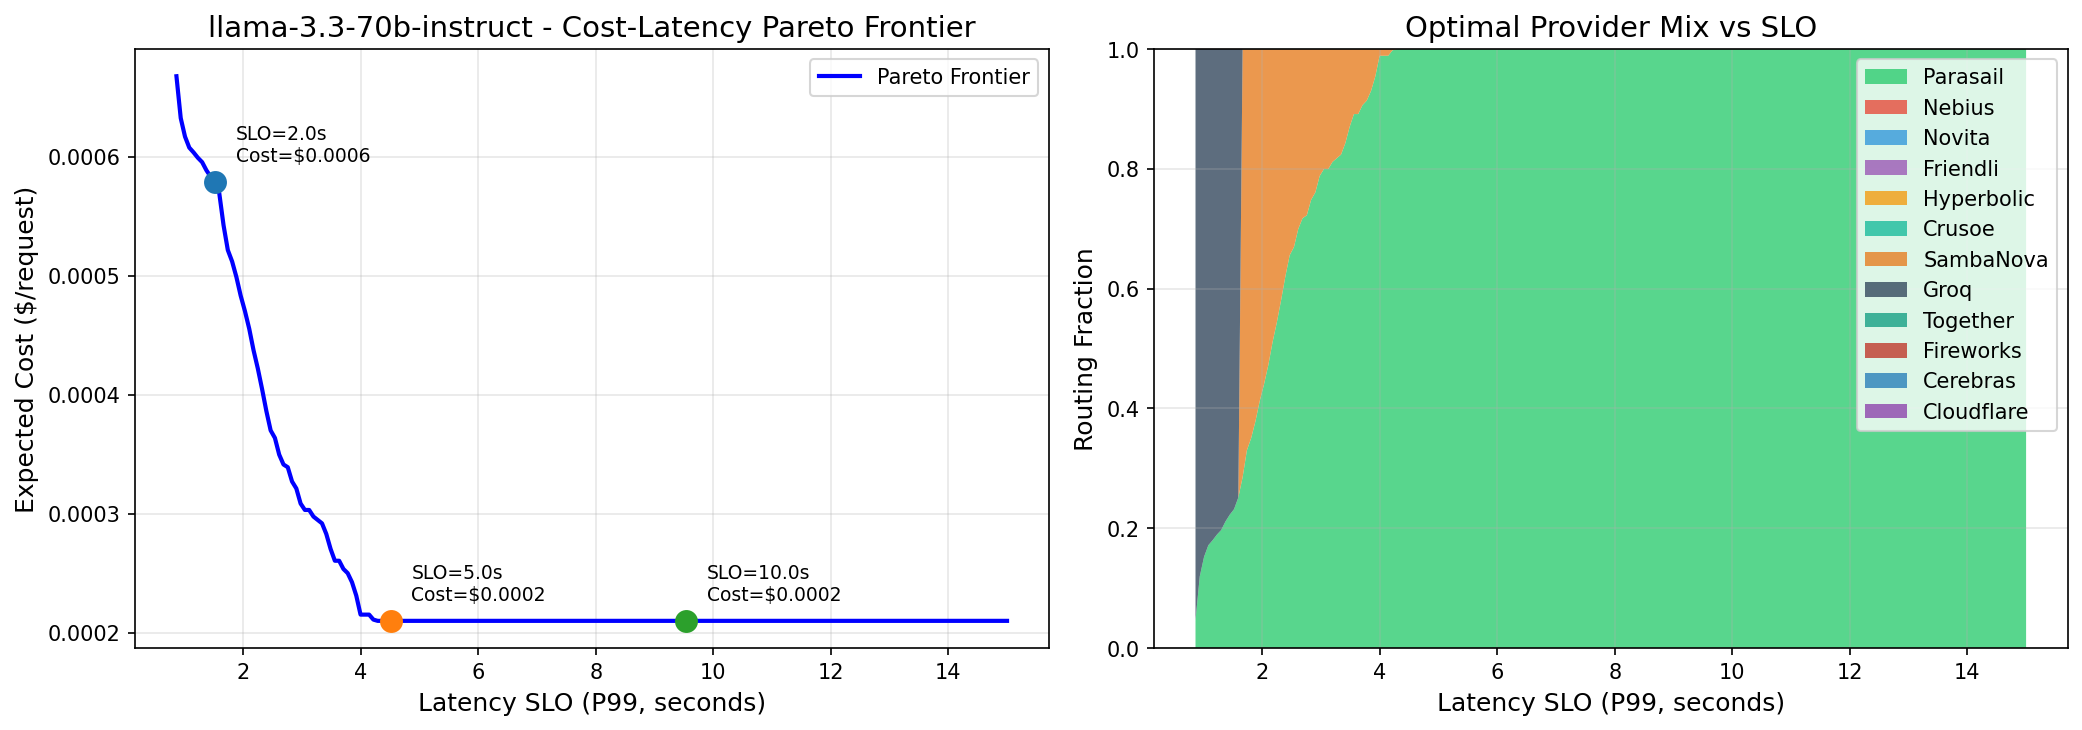
\includegraphics[width=\textwidth]{pareto_llama-3_3-70b-instruct.png}

\vspace{0.1cm}
\small
\textbf{Left:} Cost-Latency Pareto Frontier\\
\textbf{Right:} Optimal provider mix vs SLO
\end{column}
\end{columns}
\end{frame}

% ----------------------------------------------------------
\begin{frame}{Phase 2 Results: Optimal Routing Decisions}
\vspace{-0.3cm}
\begin{columns}[T]
\begin{column}{0.5\textwidth}
\centering
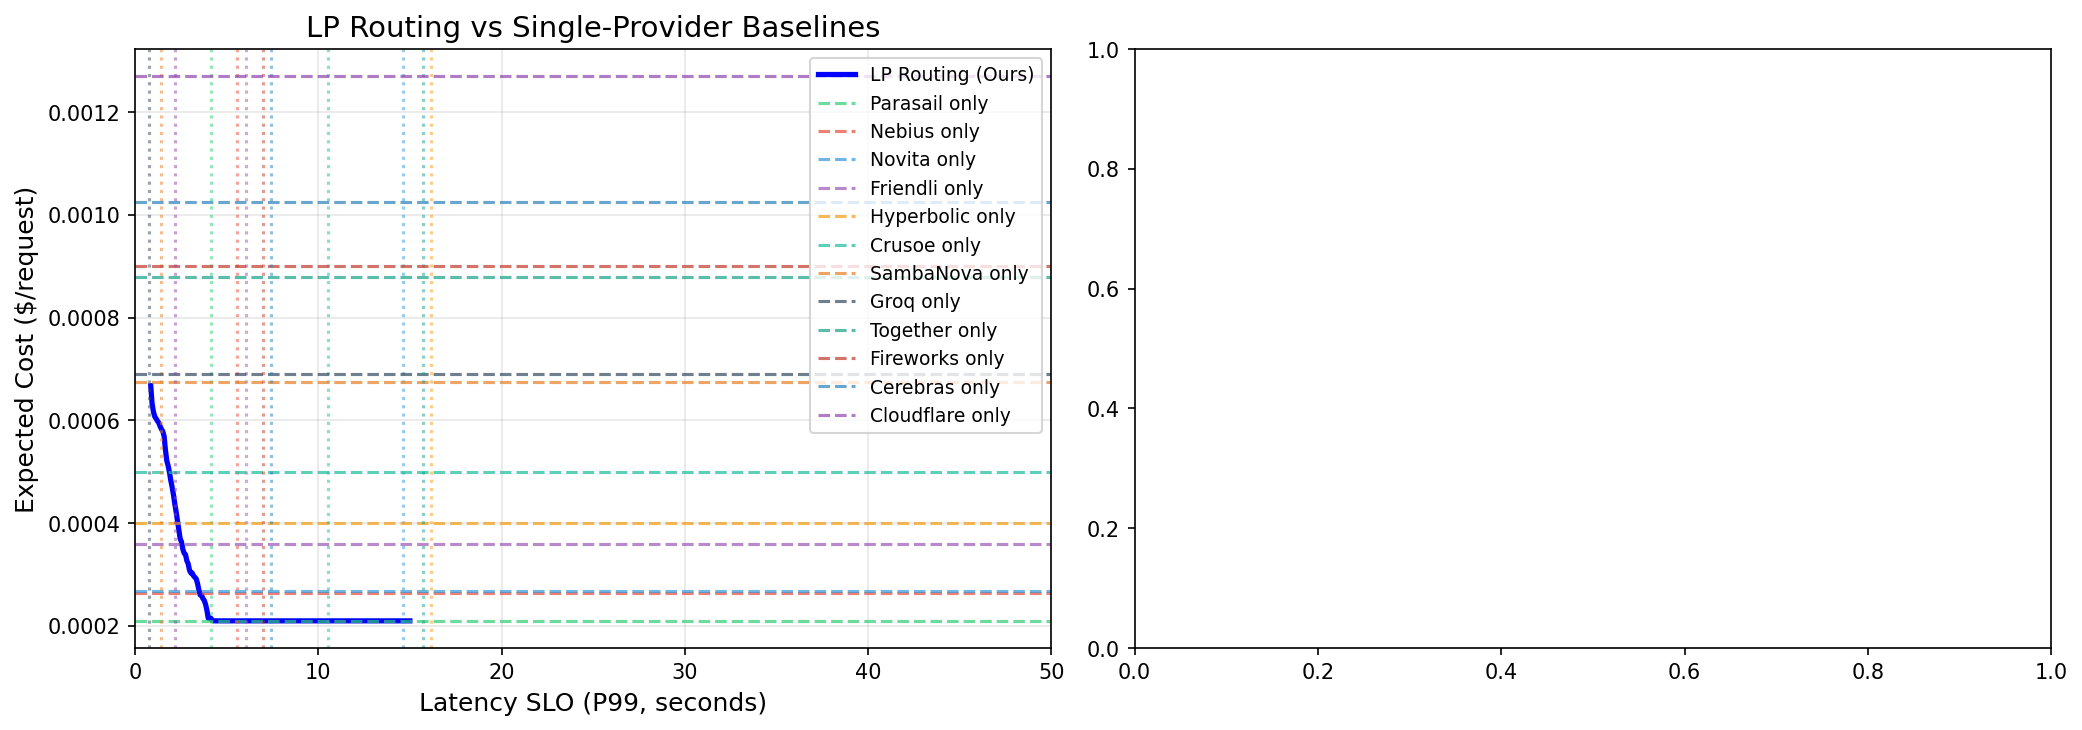
\includegraphics[width=0.95\textwidth,height=0.55\textheight,keepaspectratio]{comparison_llama-3_3-70b-instruct.png}

\scriptsize
LP routing vs single-provider baselines
\end{column}

\begin{column}{0.48\textwidth}
\scriptsize
\begin{tabular}{lcc}
\toprule
SLO & Optimal Mix & Cost \\
\midrule
2.0s & Parasail 23\% + Groq 77\% & \$0.58 \\
5.0s & \textbf{Parasail 100\%} & \$0.21 \\
10.0s & \textbf{Parasail 100\%} & \$0.21 \\
\bottomrule
\end{tabular}

\centering \tiny Cost per 1K requests

\vspace{0.15cm}
\footnotesize
\textbf{Key Findings:}
\begin{itemize}\setlength{\itemsep}{1pt}
    \item \textbf{Tight SLO} ($<$2s): Mix fast + cheap
    \item \textbf{Relaxed SLO} ($>$5s): Cheapest only
    \item \alert{70\% savings} vs Groq-only at SLO=5s
\end{itemize}
\end{column}
\end{columns}
\end{frame}

% ----------------------------------------------------------
\begin{frame}{Phase 3: Online Latency-Aware Routing}
\vspace{-0.3cm}
\begin{columns}[T]
\begin{column}{0.5\textwidth}
\footnotesize
\textbf{Challenge:} Latency distributions are \alert{non-stationary}
\begin{itemize}\setlength{\itemsep}{0pt}
    \item Provider load varies by time-of-day
    \item Need \textbf{adaptive} profiling
\end{itemize}

\vspace{0.15cm}
\textbf{Moving Window Profiler:}
\begin{itemize}\setlength{\itemsep}{0pt}
    \item Short (15 min) + Long (3h) windows
    \item Adaptive: $\beta = \frac{N_{\text{short}}}{N_{\text{short}} + \lambda}$
\end{itemize}
\[
\hat{F}(L) = \beta \cdot F_{\text{short}} + (1-\beta) \cdot F_{\text{long}}
\]
\end{column}

\begin{column}{0.48\textwidth}
\footnotesize
\textbf{Online Algorithm:}
\begin{enumerate}\setlength{\itemsep}{0pt}
    \item Update profiles with recent samples
    \item Solve LP: $\pi^* = \arg\min_\pi \sum_j \pi_j c_j$
    \item Sample provider via SWRR($\pi^*$)
\end{enumerate}

\vspace{0.15cm}
\textbf{SWRR = Smooth Weighted Round-Robin}
\begin{itemize}\setlength{\itemsep}{0pt}
    \item Deterministic sampling from $\pi^*$
    \item Exact traffic proportions
\end{itemize}
\end{column}
\end{columns}
\end{frame}

% ----------------------------------------------------------
\begin{frame}{Phase 3 Results: Online Routing Performance}
\vspace{-0.3cm}
\begin{columns}[T]
\begin{column}{0.48\textwidth}
\centering

\includegraphics[width=0.95\textwidth,height=0.45\textheight,keepaspectratio]{provider_latency_cdf.png}

\scriptsize
ECDF of TTFT (133K requests)
\end{column}

\begin{column}{0.5\textwidth}
\scriptsize
\begin{tabular}{lccc}
\toprule
Policy & Viol. & Cost & P99 \\
\midrule
Single-best & 0.4\% & \$23 & 794ms \\
Cheapest & 2.0\% & \$8 & 1438ms \\
Random & 6.6\% & \$27 & 2070ms \\
\textbf{LP-Mix} & \textbf{1.2\%} & \textbf{\$13} & \textbf{1056ms} \\
\bottomrule
\end{tabular}

\centering \scriptsize SLO=1.0s, cost per 1K requests

\vspace{0.2cm}
\footnotesize
\textbf{LP-Mix Advantages:}
\begin{itemize}\setlength{\itemsep}{1pt}
    \item \textbf{41\% cheaper} than Single-best
    \item \textbf{5x lower} violation than Random
    \item Adaptive to provider drift
\end{itemize}
\end{column}
\end{columns}
\end{frame}

% ----------------------------------------------------------
\begin{frame}{Phase 4: Smart Hedging for Tight SLOs}
\vspace{-0.3cm}
\begin{columns}[T]
\begin{column}{0.5\textwidth}
\scriptsize
\textbf{Problem:} Tail latency causes SLO violations even with optimal routing.

\vspace{0.1cm}
\textbf{Hedging:} At time $t$, if $P(\text{TTFT} > L \mid \text{TTFT} > t)$ is high, send backup.

\vspace{0.1cm}
\textbf{Survival:} $S(L \mid t) = \frac{1 - F(L)}{1 - F(t)}$

\vspace{0.15cm}
\centering
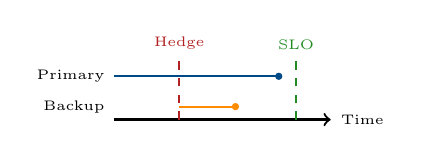
\begin{tikzpicture}[scale=0.55]
    \draw[->, thick] (0,0) -- (5,0) node[right] {\tiny Time};
    \draw[thick, icmlblue] (0,1) -- (3.8,1);
    \node[left, font=\tiny] at (0,1) {Primary};
    \filldraw[icmlblue] (3.8,1) circle (2pt);
    \draw[thick, icmlred, dashed] (1.5,0) -- (1.5,1.4);
    \node[above, font=\tiny, text=icmlred] at (1.5,1.4) {Hedge};
    \draw[thick, icmlorange] (1.5,0.3) -- (2.8,0.3);
    \node[left, font=\tiny] at (0,0.3) {Backup};
    \filldraw[icmlorange] (2.8,0.3) circle (2pt);
    \draw[thick, icmlgreen, dashed] (4.2,0) -- (4.2,1.4);
    \node[above, font=\tiny, text=icmlgreen] at (4.2,1.4) {SLO};
\end{tikzpicture}
\end{column}

\begin{column}{0.48\textwidth}
\scriptsize
\begin{tabular}{lcc}
\toprule
Strategy & Viol. & Hedge \\
\midrule
No hedging & 1.2\% & 0\% \\
Fixed timeout & 0.2\% & 11\% \\
\textbf{Smart residual} & \textbf{0\%} & \textbf{40\%} \\
Smart survival & 0\% & 60\% \\
\bottomrule
\end{tabular}

\vspace{0.2cm}
\footnotesize
\textbf{Smart residual:} 0\% violations with best cost-efficiency

\vspace{0.15cm}
\textbf{Key insight:} Hedge only when survival probability indicates likely SLO miss
\end{column}
\end{columns}
\end{frame}

% ----------------------------------------------------------
\begin{frame}{Phase 4 Results: Hedging Strategy Comparison}
\vspace{-0.3cm}
\begin{columns}[T]
\begin{column}{0.48\textwidth}
\centering
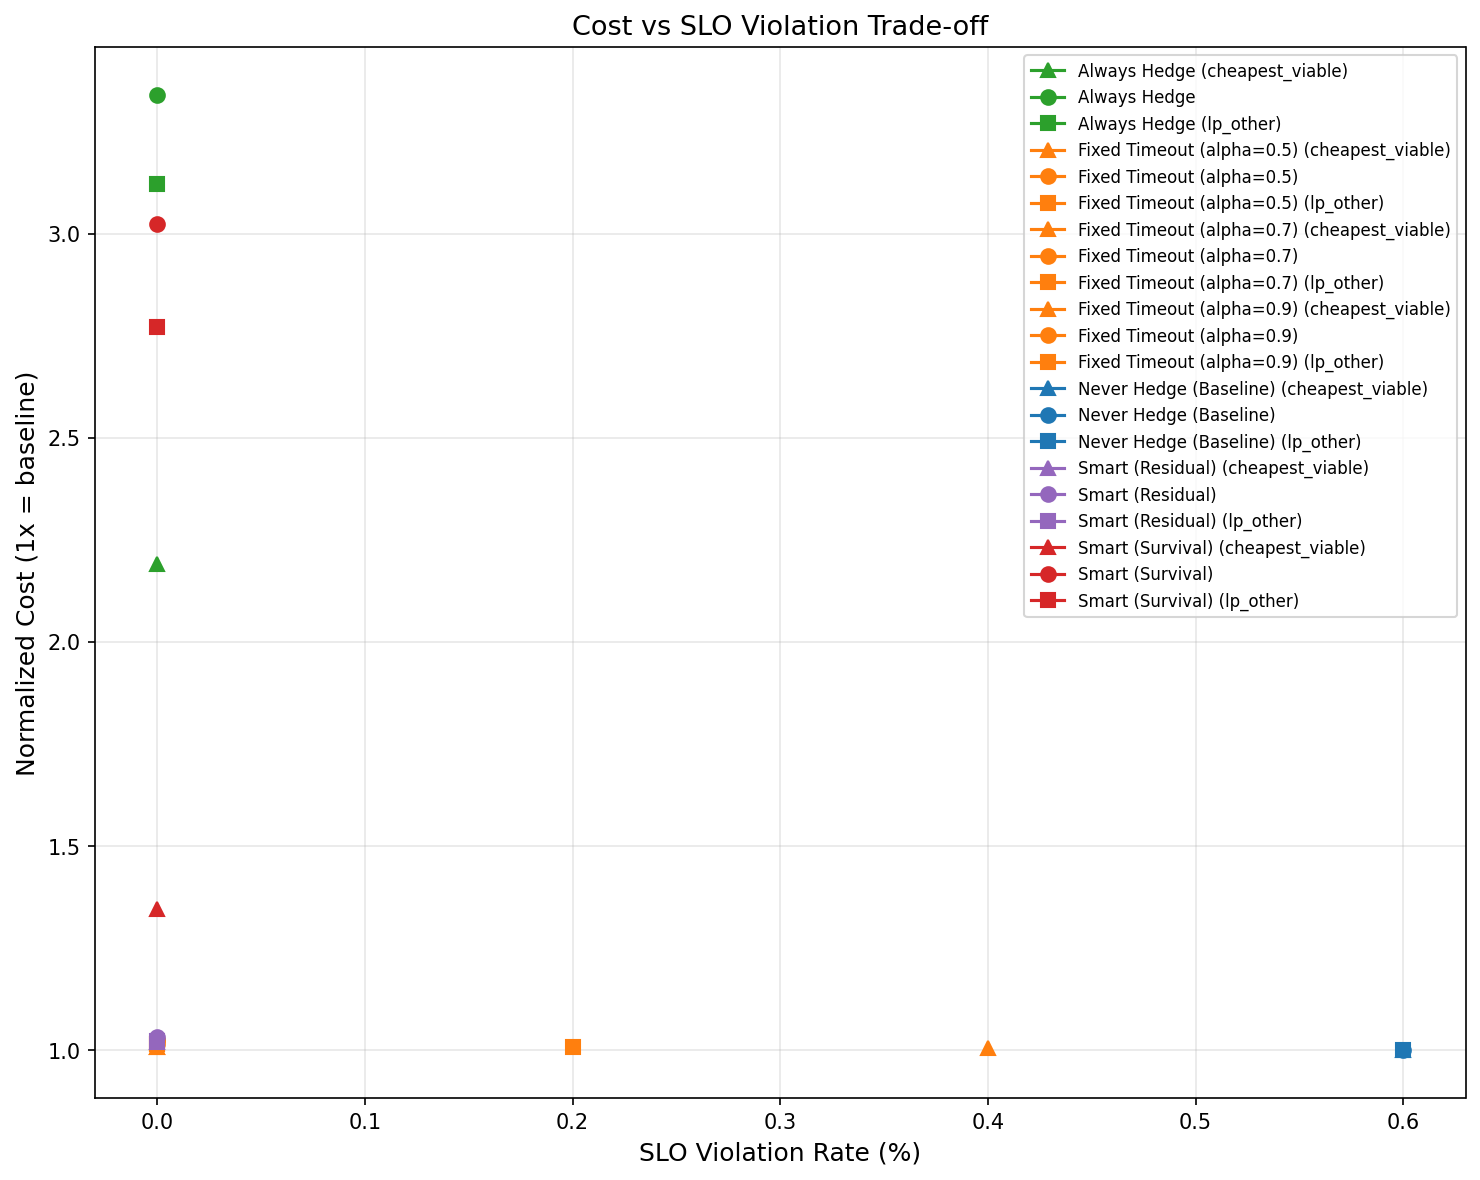
\includegraphics[width=0.95\textwidth,height=0.5\textheight,keepaspectratio]{phase4_pareto.png}

\scriptsize
Cost vs Violation Pareto Frontier
\end{column}

\begin{column}{0.48\textwidth}
\centering
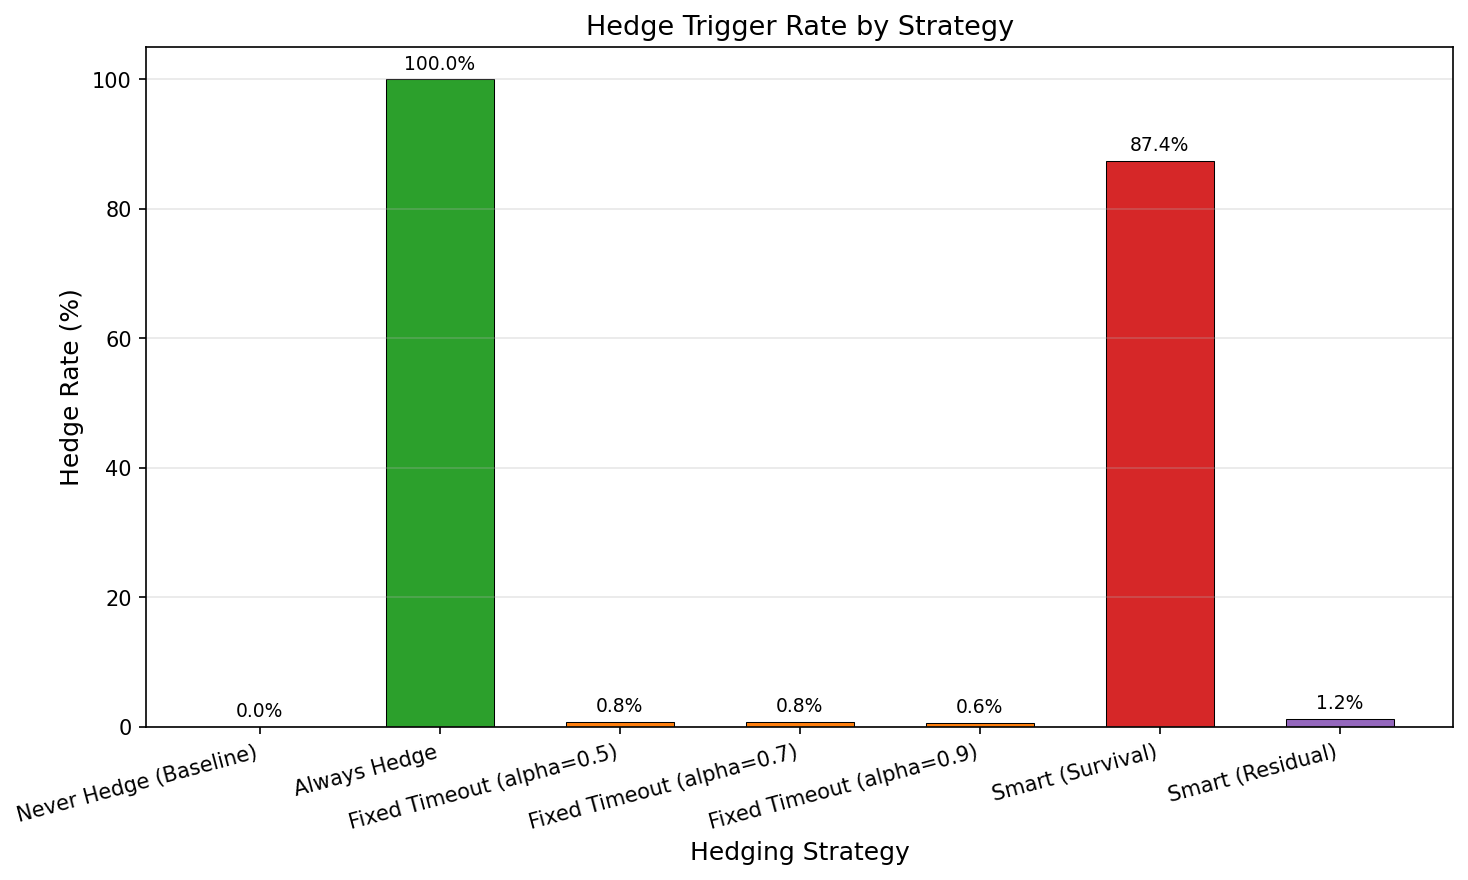
\includegraphics[width=0.95\textwidth,height=0.5\textheight,keepaspectratio]{phase4_hedge_rate.png}

\scriptsize
Hedge Rate by Strategy
\end{column}
\end{columns}

\vspace{0.15cm}
\centering
\footnotesize
\textbf{Key Finding:} \texttt{smart\_residual} achieves \textbf{0\% violations} with \textbf{40\% hedge rate}
\end{frame}

% ----------------------------------------------------------
\begin{frame}{Latency Routing: Summary}
\vspace{-0.2cm}
\begin{center}
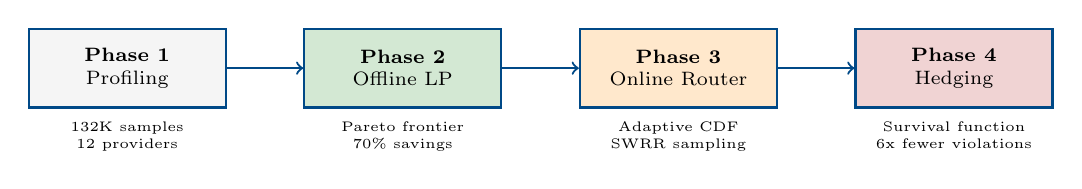
\begin{tikzpicture}[
    phase/.style={rectangle, draw=icmlblue, thick, minimum width=2.5cm, minimum height=1cm, align=center, font=\scriptsize},
    arrow/.style={->, thick, icmlblue}
]
    \node[phase, fill=lightgray] (p1) at (0,0) {\textbf{Phase 1}\\Profiling};
    \node[phase, fill=icmlgreen!20] (p2) at (3.5,0) {\textbf{Phase 2}\\Offline LP};
    \node[phase, fill=icmlorange!20] (p3) at (7,0) {\textbf{Phase 3}\\Online Router};
    \node[phase, fill=icmlred!20] (p4) at (10.5,0) {\textbf{Phase 4}\\Hedging};

    \draw[arrow] (p1) -- (p2);
    \draw[arrow] (p2) -- (p3);
    \draw[arrow] (p3) -- (p4);

    \node[below=0.05cm of p1, font=\tiny, align=center] {132K samples\\12 providers};
    \node[below=0.05cm of p2, font=\tiny, align=center] {Pareto frontier\\70\% savings};
    \node[below=0.05cm of p3, font=\tiny, align=center] {Adaptive CDF\\SWRR sampling};
    \node[below=0.05cm of p4, font=\tiny, align=center] {Survival function\\6x fewer violations};
\end{tikzpicture}
\end{center}

\vspace{0.2cm}

\begin{columns}[T]
\begin{column}{0.48\textwidth}
\footnotesize
\textbf{Key Contributions:}
\begin{itemize}\setlength{\itemsep}{1pt}
    \item \textbf{LP formulation} for latency-cost tradeoff
    \item \textbf{Online algorithm} with adaptive profiling
    \item \textbf{Smart hedging} for tail latency control
\end{itemize}
\end{column}

\begin{column}{0.48\textwidth}
\footnotesize
\textbf{Results (SLO=1s):}
\begin{itemize}\setlength{\itemsep}{1pt}
    \item \textbf{0\%} SLO violations with smart hedging
    \item \textbf{40\%} hedge rate (cost-effective)
    \item Validated on \textbf{133K} real OpenRouter requests
\end{itemize}
\end{column}
\end{columns}
\end{frame}

% ============================================================
\section{Contributions \& Future Work}
% ============================================================

% ----------------------------------------------------------
\begin{frame}{Summary of Contributions}
\begin{columns}[T]
\begin{column}{0.48\textwidth}
\begin{enumerate}
    \item \textbf{Problem Formulation}
    \begin{itemize}
        \item First formal study of hybrid LLM routing
        \item Two-stage: quota + concurrency
    \end{itemize}

    \vspace{0.2cm}
    \item \textbf{Offline Algorithms}
    \begin{itemize}
        \item Stage 1: $O(n \log n)$ closed-form
        \item Stage 2: Time-indexed ILP
    \end{itemize}

    \vspace{0.2cm}
    \item \textbf{Online Algorithms}
    \begin{itemize}
        \item Primal-Dual threshold strategy
        \item Learning-Augmented (LA-PD)
        \item CR: \textbf{1.18x} (near-optimal)
    \end{itemize}
\end{enumerate}
\end{column}

\begin{column}{0.48\textwidth}
\begin{enumerate}
    \setcounter{enumi}{3}
    \item \textbf{Ablation Study}
    \begin{itemize}
        \item 2$\times$2: Predictor $\times$ Decision Rule
        \item Finding: Predictor choice dominates
        \item EMA outperforms Histogram
    \end{itemize}

    \vspace{0.2cm}
    \item \textbf{Empirical Results}
    \begin{itemize}
        \item \textbf{30\% cost savings} vs All-API
        \item \textbf{9\% better} than Greedy
        \item 1.4M requests, 61 days
    \end{itemize}
\end{enumerate}

\vspace{0.3cm}
\centering
\fbox{\parbox{0.9\textwidth}{
\centering
\small
\textbf{Takeaway:} Simple EMA predictor + Primal-Dual\\achieves near-optimal online routing
}}
\end{column}
\end{columns}
\end{frame}

% ----------------------------------------------------------
\begin{frame}{Discussion: Real-World Subscription Complexity}
\begin{columns}[T]
\begin{column}{0.48\textwidth}
\begin{block}{Coding Plan Subscriptions}
Examples: GPT Plus, Claude Pro, GLM, MiniMax
\begin{itemize}
    \item \textbf{Prompt-based} quota (not request-based)
    \item One prompt $\approx$ 4--5 API requests
    \item Multi-tier limits: \textbf{hourly + daily + weekly}
\end{itemize}
\end{block}

\vspace{0.2cm}
\begin{exampleblock}{Example: Typical Coding Plan}
\begin{itemize}
    \item 50 prompts per 5-hour window
    \item 500 prompts per week
    \item Reset times: rolling vs. calendar-based
\end{itemize}
\end{exampleblock}
\end{column}

\begin{column}{0.48\textwidth}
\begin{block}{Mapping to Our Framework}
\begin{itemize}
    \item \textbf{Prompt} $\rightarrow$ generalized quota unit
    \item \textbf{5-hour window} $\rightarrow$ short-term $S_Q$ with $T=5h$
    \item \textbf{Weekly cap} $\rightarrow$ hierarchical quota constraint
\end{itemize}
\end{block}

\vspace{0.2cm}
\begin{alertblock}{Extension: Hierarchical Quotas}
\[
\sum_{i \in \mathcal{R}_{\text{window}}} x_i^Q \le Q_{\text{short}}, \quad
\sum_{i \in \mathcal{R}_{\text{week}}} x_i^Q \le Q_{\text{long}}
\]
Our ILP formulation naturally extends to multiple nested quota constraints.
\end{alertblock}
\end{column}
\end{columns}
\end{frame}

% ----------------------------------------------------------
\begin{frame}{}
\vspace{1.5cm}
\begin{center}
\textcolor{icmlblue}{\Huge \textbf{Questions?}}

\vspace{1cm}
\large
Code: \texttt{github.com/HarvardSys/hybridInference}

\vspace{0.5cm}
\normalsize
Harvard Systems Lab
\end{center}
\end{frame}

% ----------------------------------------------------------
% Appendix Slides
% ----------------------------------------------------------
\appendix

\begin{frame}[noframenumbering]{Appendix: Gutter Pool (Local GPU Deployment)}
\begin{columns}[T]
\begin{column}{0.55\textwidth}
\textbf{What is a Gutter Pool?}
\begin{itemize}
    \item Pool of \textbf{spare GPU nodes} kept hot/idle
    \item Primary purpose: \alert{High Availability}
    \item When a serving node fails $\rightarrow$ gutter node takes over
\end{itemize}

\vspace{0.3cm}
\textbf{Why Model as Quota-Based ($S_Q$)?}
\begin{itemize}
    \item Fixed pool size $\approx$ daily quota $Q$
    \item Zero marginal cost (already provisioned)
    \item Limited capacity (can't overuse)
\end{itemize}
\end{column}

\begin{column}{0.4\textwidth}
\centering
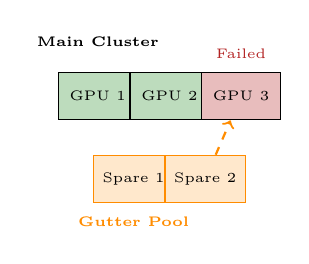
\begin{tikzpicture}[scale=0.7,
    node/.style={rectangle, draw, minimum width=1cm, minimum height=0.6cm, font=\tiny},
    gutter/.style={rectangle, draw=icmlorange, fill=icmlorange!20, minimum width=1cm, minimum height=0.6cm, font=\tiny}
]
    \node[node, fill=icmlgreen!30] (n1) at (0,1.5) {GPU 1};
    \node[node, fill=icmlgreen!30] (n2) at (1.3,1.5) {GPU 2};
    \node[node, fill=icmlred!30] (n3) at (2.6,1.5) {GPU 3};
    \node[above=0.05cm of n3, font=\tiny, text=icmlred] {Failed};

    \node[gutter] (g1) at (0.65,0) {Spare 1};
    \node[gutter] (g2) at (1.95,0) {Spare 2};

    \node[above=0.2cm of n1, font=\tiny\bfseries] {Main Cluster};
    \node[below=0.05cm of g1, font=\tiny\bfseries, text=icmlorange] {Gutter Pool};

    \draw[->, thick, icmlorange, dashed] (g2) -- (n3);
\end{tikzpicture}

\vspace{0.2cm}
\small
Our algorithms apply to local GPU scheduling too!
\end{column}
\end{columns}
\end{frame}


\begin{frame}[noframenumbering]{Appendix: Time-Indexed ILP Details}
\textbf{Concurrency Constraint (Linearized):}
\begin{equation*}
\sum_{i \in \mathcal{R}} \sum_{\tau=\max(\alpha_i, t-\hat{p}_i+1)}^{\min(\beta_i, t)} z_{i,\tau} \leq C, \quad \forall t \in \{0, \ldots, T\}
\end{equation*}

\vspace{0.3cm}
\textbf{Variable Count:}
\begin{itemize}
    \item Routing: $3n$ binary variables
    \item Scheduling: $O(n \cdot T / \Delta)$ binary variables
    \item Trade-off: finer $\Delta$ $\Rightarrow$ more accurate but larger problem
\end{itemize}
\end{frame}

\begin{frame}[noframenumbering]{Discussion: Paper Title Candidates}
\begin{enumerate}
    \item \textbf{From Offline Oracles to Online Thresholds:} \\
    Cost-Optimal Hybrid LLM Routing

    \vspace{0.3cm}
    \item \textbf{Beyond Pay-per-Token:} \\
    Cost-Optimal LLM Routing under Subscription Plans

    \vspace{0.3cm}
    \item \textbf{\textcolor{icmlblue}{HybridRoute}:} \\
    Cost-Optimal LLM Routing with Quota and Concurrency Constraints

    \vspace{0.3cm}
    \item \textbf{Cost-Optimal LLM Routing} \\
    Across Subscription and Pay-per-Token Providers
\end{enumerate}

\vspace{0.4cm}
\small
\textit{Considerations: ICML style (algorithm-focused), searchability (LLM, routing, cost), length for proceedings}
\end{frame}

\end{document}
